\documentclass[11pt,a4paper,draft]{report}

% twoside,openright screws up sideways figure positioning, use empty pages
% to force openright formating by hand.
% The PDF must be named rep_grochmalm_act.pdf

\usepackage[utf8]{inputenc}
\usepackage[T1]{fontenc}
\usepackage{textcomp}

\usepackage{parskip}
\usepackage{multicol}
\usepackage{titlesec}
\usepackage{fancyhdr}
\usepackage{fancyvrb}

\usepackage{amsmath}
\usepackage{amssymb}
\usepackage{tocloft}
\usepackage{graphicx}
\usepackage{rotfloat}
\usepackage{multirow}
\usepackage{booktabs}
\usepackage{longtable}
\usepackage[table]{xcolor}

% \label convention
% chap:    chapter
% sec:     section
% subsec:  subsection
% fig:     figure
% tab:     table
% eq:      equation
% lst:     code listing
% itm:     enumerated list item
% app:     appendix subsection

\title{Style Based Drawn Artwork Image Classification}
\author{A dissertation submitted in partial fulfilment of the requirements\\
  for the MSc in Intelligent Technologies\\
  \\
  by Michal Grochmal
  $<$\href{mailto:grochmal@member.fsf.org}{grochmal@member.fsf.org}$>$\\
  supervisor Dell Zhang
  $<$\href{mailto:dell@dcs.bbk.ac.uk}{dell@dcs.bbk.ac.uk}$>$\\
  \\
  Department of Computer Science and Information Systems\\
  Birkbeck College, University of London
}
\date{September 2014}

\usepackage[colorlinks=true]{hyperref}

%\hyphenation{ge-ne-ric Ge-ne-ric Ro-me-ro Ma-ria}

% fix adobe's PDF reader (it cannot stand xcolor)
\definecolor{lightgray}{gray}{0.7}
\setlength{\headheight}{16pt}
\setlength{\arrayrulewidth}{0.6pt}

%\renewcommand{\chaptername}{Section}  % Not needed
\renewcommand{\bibname}{References}
\titlespacing*{\chapter}{0pt}{60pt}{60pt}

\titleformat{\chapter}[display]{
  \normalfont\huge\bfseries}{\chaptertitlename\ \thechapter}{20pt}{\Huge}
\titleformat{\section}[block]{
  \normalfont\Large\bfseries}{\thesection}{1em}{}
\titleformat{\subsection}[block]{
  \normalfont\large\bfseries}{\thesubsection}{1em}{}

\begin{document}
\VerbatimFootnotes
\maketitle

\newpage
\null
\thispagestyle{empty}
\newpage

\pagestyle{fancy}
\lhead{}
\chead{STYLE BASED DRAWN ARTWORK IMAGE CLASSIFICATION}
\rhead{}

\begin{abstract}

The abstract of the work, this will be written at the very end

\begin{flushright}
\emph{Ars longa, vita brevis -- Hippocrates}
\end{flushright}
\end{abstract}

\newpage
\null
\thispagestyle{empty}
\newpage

\newpage
\phantomsection
\addcontentsline{toc}{chapter}{Table of Contents}
\setcounter{page}{1}
\pagenumbering{roman}
\tableofcontents

\newpage
\phantomsection
\addcontentsline{toc}{chapter}{List of Figures}
\listoffigures

\newpage
\null
\thispagestyle{empty}
\newpage

\newpage
\phantomsection
\addcontentsline{toc}{chapter}{List of Tables}
\listoftables

\newpage
\null
\thispagestyle{empty}
\newpage

\newpage
\phantomsection
\addcontentsline{toc}{chapter}{Academic Declaration}
\chapter*{Academic Declaration}
This report is substantially the result of my own work except where explicitly
indicated in the text.  I give my permission for it to be submitted to the JISC
Plagiarism Detection Service.  I have read and understood the sections on
plagiarism in the Programme Handbook and the College website.

The report may be freely copied and distributed provided the source is
explicitly acknowledged.

\newpage
\null
\thispagestyle{empty}
\newpage

\newpage
\phantomsection
\addcontentsline{toc}{chapter}{Acknowledgements}
\chapter*{Acknowledgements}
Thanks to my family and my friend, for their patience with me not having the
time to spend with them.

\newpage
\null
\thispagestyle{empty}
\newpage

\newpage
\setcounter{page}{1}
\pagenumbering{arabic}

\chapter{Introduction}
\begin{multicols}{2}

Similar images are classified by Content Based Image Retrieval systems (CBIR
systems) based on \emph{several features}.  The feature we use depend on one of
the meanings (semantics) contained in the image, it could be one specific
object present in the image, a combination of objects, a specific person or
something even different.  One image has often much more than one meaning.
e.g. we might query a collection of personal photos using a picture of our
cousin holding a carnival mask in Venice.  For this query image we might ask:
whether there are photos of our cousin in the collection, or whether there are
photos of venetian carnival masks, or photos with a specific building or
location in Venice in the background.

Different \emph{sets of features} are needed for different semantics and
different collections.  In this work we will search for features related to the
\emph{artistic style} between different artists and, more generally between
different art schools (aka. art movements).  We will focus on \emph{aesthetics}
of an image as it is related to the concept of art \cite{rmc12ajs}, and on the
\emph{emotions} an image can provoke on the viewer as it is one of the purposes
of art \cite{mach10clas}.

CBIR systems for artwork \cite{cfsp12air,isv12mpeg,ymvz03tree} can benefit from
extra features and from a better understanding of current features.  Museum
collection can also benefit from better classification of art images:  Several
images in these collections miss some or all metadata, by finding similar
images we could fill in the missing metadata.

\section{Background}

Features that are independent for objects in the image (or at least as
independent as possible) need to be used to evaluate the art style.  Work by
Zirnhelt \cite{zirnhelt07art} present a limited number of such features in the
\emph{context of art}.  Works by Machaijdik \cite{mach10clas} and Romero
\cite{rmc12ajs} present more features independent from objects, but most of the
features tried were tested on illustration and photography only.  Romero in
\cite{rmc12ajs} tests some of the features on a very limited number of art
paintings.  Thanks to photo web sharing (\texttt{photo.net},
\texttt{panoramio.com} or \texttt{flickr.com}) consistent datasets of
photography are much easier to acquire than datasets of art, that is the major
reason why the majority of work on style uses photography.

Art paintings style is evident to humans, Figures \ref{fig:diff} and
\ref{fig:similar} show an example of image similarity.  In Figure \ref{diff} we
see paintings by Francesco Granacci and by Francesco Pesellino, these paintings
contain similar object and depict a similar contex yet their \emph{style is
different}.  Figure \ref{fig:similar} shows two paintings by Delacroix, in
which the \emph{style is similar} although the scenes depicted are different.
Using the correct features we shall be capable of identifying the firs two
images as different and the last two as similar.  [The images are part of the
public collection of the Victoria and Albert Museum in London, this collection
is used as a dataset in this work.  See Chapter \ref{chap:data}.]

To achieve such classification we follow works that detour from interest points
or corner detection for general object identification as SIFT or MSER
techniques \cite{szel11book}.  Such features describe the content of the image
instead of it's style.

\begin{figure*}[tb]  % figure* instead of figure because of multicols
\centering
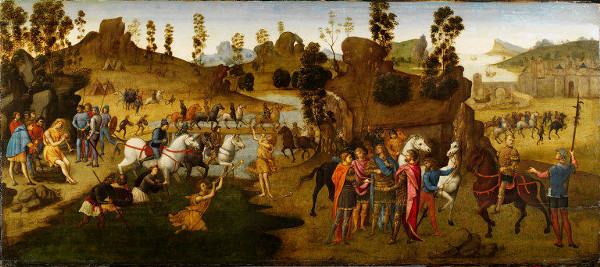
\includegraphics[width=0.48\textwidth]{diff_caesar}
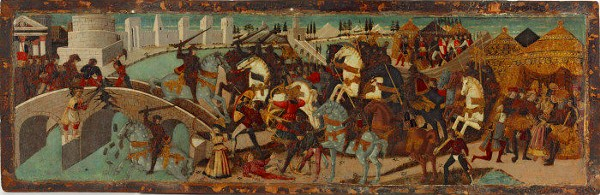
\includegraphics[width=0.48\textwidth]{diff_horatius}
\caption[Example of different styles]{The image to the left is the painting
"Julius Caesar and the Crossing of the Rubicon" by \emph{Francesco Granacci}
and to the right is the panel "Horatius Cocles Defending the Sublician Bridge"
by \emph{Francesco Pesellino}.  The theme in both images is the same: roman
warfare, soldiers and horses moving through a river.  Yet the style used in
depicting both scenes is different.}
\label{fig:diff}
\end{figure*}

\begin{figure*}[tb]
\centering
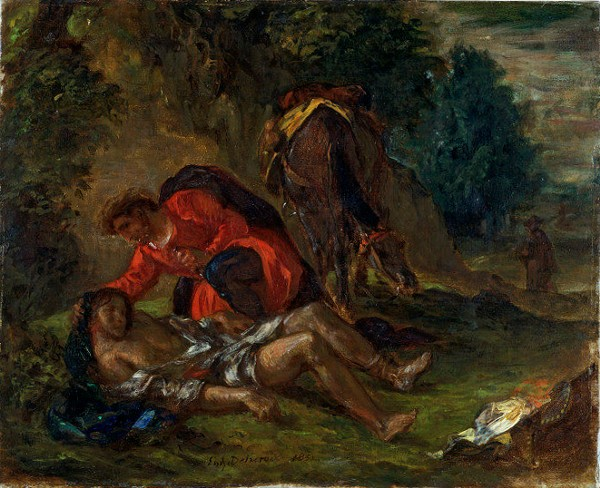
\includegraphics[width=0.48\textwidth]{sim_delacroix_samaritan}
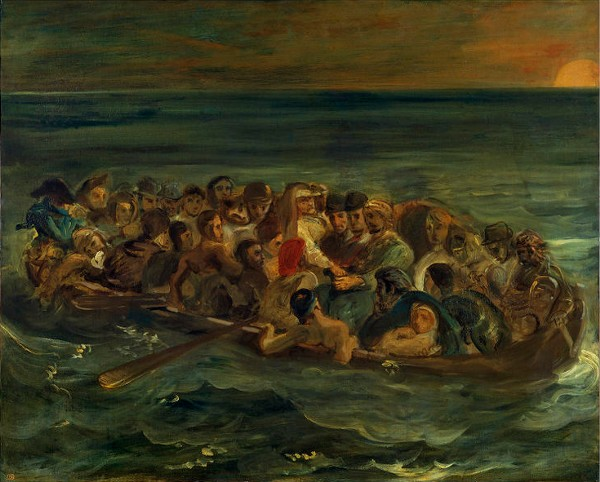
\includegraphics[width=0.48\textwidth]{sim_delacroix_shipwreck}
\caption[Example of similar styles]{A similar style can be observed in these
two paintings by \emph{Eug\`ene Delacroix}: "The Good Samaritan" (left) and
"The Shipwreck of Don Juan" (right).  The author's style of painting is
observed in both paintings, although the theme of the images is completely
different.}
\label{fig:similar}
\end{figure*}

\section{Features in the previous works}

A richer sets of features can be found in works that explore style in
photography \cite{jma12clas,cmrc13fs,rmc12ajs,mach10clas}.  \emph{Image
complexity} based on lossy compression, \emph{standard deviation} and
\emph{average} over components of \emph{HSV} and/or \emph{HSL} colour
representation, \emph{Itten colours and contrasts} and weighted importance of
all these feature in the center of the image.  Other works propose histograms
of black and white on drawing classification \cite{kroner98draw} or MPEG-7
descriptors as features.

Size normalisation of all images is needed as all these features are
\emph{scale dependent} \cite{jma12clas,mach10clas}.  Also, several of the works
(\cite{jma12clas,cmrc13fs,rmc12ajs}) perform colour normalisation to eliminate
the differences of illumination between images.  RGB colour space do not
represent well the human perception of the image \cite{mach10clas} therefore
the features are extracted from the \emph{HSV} and \emph{HSL} colour
representations of the image.

In this work, to the features used by Romero in \cite{rmc12ajs} we add many
features described by Machajdik in \cite{mach10clas}.  Although we ignore some
of Machajdik's features that are directly related to object recognition as we
need features that are as independent as possible form the objects in the
image.  From \emph{Romero's work} we use Kolmogorov complexity features and
image averages, from \emph{Machajdik's work} we use Itten colours, Itten
contrasts, grey level co-occurrence matrix and the rule of thirds.  The most
complex of these features to implement are the Itten contrasts.  In Romero's
and Machajdik's work the task of author classification is not the main focus,
we use their features on a much bigger collection as a main focus of this work.
We also extrapolate the \emph{feature extraction and classification} to
classify on artistic schools.

\section{Project execution}

Time and effort to acquire the datasets proved to be the most complicated part
of the work.  It is not surprising that the number of works that explore art
collections is small given that big and consistent datasets are hard to
acquire.  The remaining of the time of the project was spent on feature
extraction, classification and write up.

The \emph{13 weeks} of the project were executed as follows: First 7 weeks were
used for dataset acquisition and cleansing, next 3 week for feature extraction,
one week of holiday, 1 week of classification and 1 week for write up.  The
dataset acquisition work can be subdivided into: \emph{1st week}: reading the
VAM JSON API and building scripts for the VAM dataset crawlers; \emph{2nd
week}: organisation of VAM data, removing inexistent, duplicated, misclassified
paintings and unknown artists;  \emph{3rd week}: writing crawlers for the NIRP
dataset, crawlers over artist indexes and painting indexes which are then
compared against each other;  \emph{4th week}: Word count and manual selection
of artists from the NIRP dataset;  \emph{5th week}: Recording of data from NIRP
dataset, including manual intervention with encoding issues;  \emph{6th week}:
writing unixjsons tools (see Appendix \ref{chap:unixjsons} to deal with data
organisation;  \emph{7th week}: using unixjsons tools to filter only the images
of artists that have a sizeable amount of paintings, also a manual check on the
resulting images.

Feature extraction can be subdivided into: \emph{8th week}: normalisation,
separation and Kolmogorov complexity features;  \emph{9th week}: GLCM features,
rule of thirds and image averages; \emph{10th week}: Watershed segmentation and
Itten colours and contrasts.

Remaining two weeks were used to link metadata to the features and run the
classifiers.  The last week was mostly used to finish the report write up.

\section{Summary}

Chapter \ref{chap:data} describes the process of dataset acquisition, for each
of the two datasets used.  Chapter \ref{chap:approach} extensively describes
the feature extraction process, dividing the features into related groups and
explaining each.  Chapter \ref{chap:results} describes a crude classification
process as an example of how these features can be used.  Appendices show how
to use the code accompanying this report and show the most important parts of
the data and code used.

\end{multicols}

\chapter{Data}
\label{chap:data}

\begin{multicols}{2}

We use online art collections as the datasets for our classification,
unfortunately such art collections are far from being machine readable inputs
of images and metadata.  Two such collections are used: the \emph{Victoria and
Albert Museum (VAM)} collection\footnote{\href{http://www.vam.ac.uk/}
{http://www.vam.ac.uk}}, which is freely available for academic use.  And the
\emph{NICE paintings (NIRP)} collection available from the Visual Arts Data
Service (VADS)\footnote{\href{http://vads.ac.uk/}{http://vads.ac.uk}} project.
NIRP collection is an agglomeration of several collections of paintings
including, among others, the CACHe project\footnote{
\href{http://www.bbk.ac.uk/hosted/cache/}{http://www.bbk.ac.uk/hosted/cache}}
at the Birkbeck College.

To produce a machine readable dataset we crawl the NIRP and VAM collections for
paintings, then we filter them based on the completeness and \emph{consistency
of the metadata} of the collection item.  This task often cannot be done
automatically, e.g. we rejected a painting by Leonardo da Vinci painted in
1856, 200 years after the painter's death.  In this case it is clear that the
metadata of the item is incorrect and the painting cannot be used, but writing
a piece of software that evaluates such metadata to be correct or incorrect is
a project in it's own.  Therefore, a lot of the work on the acquisition of the
collection items was done manually as item with wrong metadata would add extra
complexity to the classification.

Results of the crawl, the images, are assigned the surname of the artist and a
unique identifier consisting of letters and numbers \texttt{<painter>\_<id>}.
We use more than one dataset, therefore later the images are prefixed with the
dataset name to generate globally unique identifiers:
\texttt{<dataset>\_<painter>\_<id>} (e.g. \texttt{vam\_constable\_2006AP4487}
or \texttt{nirp\_monticelli\_fa000286}).

\section{Victoria and Albert Museum (VAM)}

In the VAM collection we are interested in the collection objects classified as
paintings.  The entire collection contains other objects that are not
paintings: sculpture, clothing or manuscripts among others.  In the VAM
collection there are 2000 items classified as paintings.  VAM exposes a JSON
API\footnote{\href{http://www.vam.ac.uk/api/json/museumobject/}
{http://www.vam.ac.uk/api/json/museumobject/}} to retrieve metadata and image
web locations, the metadata is organised as a small JSON structure for each
museum item.

The API do not allow to retrieve data for more than 45 items in one call,
therefore we develop a crawling script (\texttt{vam-get-all.py}) that retrieves
data about the 2000 paintings in order.  Instead of working with big JSONs by
joining all JSON results into one agglomerated result we take the approach of
Chen in \cite{chen09yahoo} and use a plain text file containing one small JSON
per line.  Each line in this JSONS file is the JSON encoded data for one
painting, as Chen \cite{chen09yahoo} describes, this approach reduces the
memory needed to process each record and allows the processing of the entire
dataset as a stream.

To easily work with files in the JSONS, format we developed implementations of
the \texttt{grep}, \texttt{cut}, \texttt{sed}, \texttt{echo} and \texttt{join}
commands over files and streams in the JSONS format.  This set of tools is
described in Appendix \ref{chap:unixjsons}.

Using \texttt{jgrep} we filtered out of the collection items classified as
paintings all items that did not have and image.  This left us with 878 items
with an image.  We then downloaded the images for these items using another
crawling script (\texttt{vam-img-get.py}).  Some of the images did not depict
paintings, therefore we manually went through each of the 876 downloaded images
and removed items that were misclassified as paintings.  We found 4 images of
vases, 3 images of sculptures and 3 references to a photo of three vials of
paint (which also explained why we got 876 images for 878 items).  We removed
all misclassified items from the set and 868 paintings remained.

Several paintings had the "artist" metadata field set as: "Unknown", "unknown"
or "" (empty).  We removed all these paintings from the set as we would not be
able to evaluate the classification according to \emph{artist identification}
if we do not know the artist in the first place.  303 were removed from the set
for having the artist unknown, leaving 565 paintings with assigned artists.

Next we needed to remove artists that have a number of paintings too little to
be relevant.  A classifier that can assign the only painting of a certain
artist to that artist is not a general classifier.  Yet first, the metadata in
the "artist" field needed to be cleaned to find the names of artists and the
paintings by each artist.  e.g. the name of Charles Robert Leslie is encoded in
the VAM collection as both "Charles Robert Leslie" and "Leslie, Charles Robert
(RA)" of the name of William Mulready is encoded as "Mulready, William (RA)"
and as "Mulready, William".  A simple \texttt{jsed} script
(\texttt{cleanse-artists.jsed}) was created to re-encode the artist's names in
a consistent manner across the set of 565 paintings.

After the cleaning of artist names we got a list of 281 artists, most of them
with only one painting in the collection.  We filtered out all artists with 6
paintings or less from the set and collected the paintings for all remaining
artists.  This leaves the \emph{VAM dataset} with 193 paintings by 14 artists:
John Constable (39 paintings), Thomas Gainsborough (13 paintings), Charles
Robert Leslie (10 paintings), William Mulready (10 paintings), George Frederick
Watts (10 paintings), William Carpenter (9 paintings), Abanindranath Tagore (7
paintings), Basawan (11 paintings), Jagan (9 paintings), Kesav Kalan (15
paintings), La'l (19 paintings), Miskin (15 paintings), Tulsi Kalan (10
paintings) and Devi (16 paintings).

Table \ref{tab:crawl} shows the VAM dataset acquisition in perspective.

\begin{table*}[ptb]
\centering
\rowcolors{1}{}{lightgray}
\begin{tabular}{|l|rr|}
\toprule
Dataset & VAM dataset & NIRP dataset \\
\midrule
Paintings available                   & 2000 & 24373 \\
Unique paintings (according to index) & 2000 &  9181 \\
Paintings without an image            & 1132 &  2511 \\
Paintings with an image               &  878 &  6641 \\
Object misclassified as painting      &   10 &     1 \\
Corrupted image file                  &    0 &     8 \\
Duplicate image                       &    0 &     5 \\
Different photo of the same painting  &    0 &    15 \\
Artist of painting was not known      &  303 &   144 \\
% VAM had "Unknown", "unknown" and ""
% NIRP was a mess, as always
\midrule
Indexed artists                       &  281 &  3222 \\
Missing artist index                  &    0 &     1 \\
Not artist index entry                &    0 &     9 \\
Artists without paintings             &    0 &    23 \\
Artists used for selection            &  281 &  3190 \\
Selected artists                      &   14 &    42 \\
\midrule
Paintings by the selected artists     &  193 &  1007 \\
\bottomrule
\end{tabular}
\caption[Dataset acquisition]{Dataset acquisition.  The number of images and
artists at each phase of crawling and cleansing the dataset.}
\label{tab:crawl}
\end{table*}

\section{Visual Arts Data Service - NICE Paintings (NIRP)}

NIRP is an agglomeration of public collections in the UK and it contains more
than 9000 pre-1900 European \emph{oil paintings}.  Unfortunately the
organisation of the collection is poor, and no API exists.  The crawlers
collection the data from the NIRP collection are \emph{HTML crawlers}, yet to
maintain consistency with the VAM dataset the final form of the metadata for
the NIRP collection are plain files containing a JSON on each line.

Although no API exist for the NIRP dataset there is an alphabetical index of
artist names.  With a script (\texttt{all-artists.py}) we crawled the index of
artist names producing a list of all 3222 artists in the NIRP collection.
A manual intervention was needed in the crawl as the index for the letter "x"
exists although there is no artist name starting with the letter "x".  From the
remaining index entries we manually removed 9 entries that were not artists but
agglomerations of artists by country (e.g. "French Painters" under the letter F
or "Italian Painters" under the letter I).

Each index entry links the artist name to a query search string using the
VADS's website\footnote{\href{http://www.vads.ac.uk/collections/NIRP/index.php}
{http://www.vads.ac.uk/collections/NIRP/index.php}} search engine.  The search
retrieves matches on all words of the query, therefore the index links of the
three Italian artists: Francesco Bassano, Leandro Bassano, and Jacopo Bassano
il vecchio result in the same list of paintings for each.  Whether an artist
shares part of his name with another artist the result for both are displayed
when following the index link for any of them, e.g. every John is assigned the
paintings of all Johns in the NIRP collection.

The descriptions of paintings in the NIRP collection posses \emph{unique IDs},
therefore we collected all painting descriptions from all artists in the artist
name index including several duplicates.  With the duplicates we had 24 373
painting descriptions, filtering them by the \emph{unique IDs} resulted in 9181
unique painting descriptions.  Also, from the index of artist names we manually
removed 23 artists for which the index did not return any paintings, duplicates
of not.  This was checked using a combination of \texttt{curl} and
\texttt{grep} calls.

From the 9181 descriptions of paintings only 2511 had available images, which
we downloaded using a \texttt{get-painting.py} script.  The remaining 6641
painting descriptions were removed from the set, as we need an image of the
painting to extract features from.  A script (\texttt{by-artist.py}) was used
to crawl the descriptions of the 2511 paintings with an image, yet it did not
produce acceptable results.  The encoding of the HTML encoding used by VADS is
\texttt{UTF-8} but several pieces of metadata are encoded in \texttt{ISO
8859-1} character encoding, sometimes in \texttt{ISO 8859-2} character encoding
and some (not all) quotes are encoded in \texttt{Windows-1252} character
encoding.  The main piece of metadata which had mixed encodings across
different painting descriptions was the artist field, the most important
metadata field for this project.  The \texttt{by-artist.py} was extended to
deal with mixed encoding of \texttt{UTF-8} and \texttt{ISO 8859-1}, but the
cases where characters were encoded in \texttt{ISO 8859-2} or
\texttt{Windows-1252} needed to be dealt with manually.  After all changes, all
painting descriptions were converted to \texttt{UTF-8} character encoding and
formatted in the same way as metadata from the VAM collection (a JSONS file).

In possession of 2511 paintings with descriptions there were 3190 artists to
assign to them based on a messy artist name index.  The (now UTF-8 encoded)
data for the "artist" field was not possible to clean with a \texttt{jsed}
script as in case of the VAM collection.  Most of the data was encoded in
natural language, for example:

\begin{quote}
"artist": " Attributed to school of Masaccio (Italian painter, 1401-1428)
Attributed to Giovanni di Ser Giovanni Guidi (Italian painter, 1406-1486)
Previously attributed to Boccati, Giovanni di Piermatteo da Camerino (Italian
painter, born ca.1420, active 1480) "
\end{quote}

Even unknown artists were not stated in a machine readable way:

\begin{quote}
"artist": " Unknown  Previously attributed to Soldi, Andrea (Italian painter,
ca.  1703-1771, active in Great Britain) "
\end{quote}

Therefore the number of paintings of unknown artists for the NIRP collection in
Table \ref{tab:crawl} is smaller than the real number.

To find the actual artists of the 2511 paintings we concatenated together the
data of the "artist" field for all and run a word count algorithm over the
result.  The word count was just a combination of \texttt{jcut}, \texttt{cut},
\texttt{sed}, \texttt{sort} and \texttt{uniq} commands.  From the result of the
word count we removed stop words and removed any words appearing less than 10
times (unless the word was clearly the surname of a well known painter).  The
resulting ~2000 words were checked by hand, using \texttt{jgrep} to ensure that
it is a surname or forename of an artist by checking the "artist" metadata
field of each image that cntains that word.  It was a humongous manual work to
organise the words into 42 artist names which had a considerable number of
works in th NIRP collection.

For the selected 42 artist, a script (\texttt{filter-artists.sh}) was developed
to pick the images of each artist (using regular expressions and
\texttt{jgrep}) and to enhance the metadata with a machine readable "artist"
field.  At the end of the process each artist had a metadata file in JSONS
format and a directory of all images listed in the metadata file.  Finally, the
image file names and IDs were all converted to lowercase, to make them more
consistent.  The total of images for all the 42 artists was 1036.  The names of
all artists are too long to list therefore are presented in Table
\ref{tab:style}, together with the 14 artists from the VAM collection.

The 1036 paintings were checked for duplicates using a \texttt{SHA1} checksum,
resulting in 8 corrupted files and 5 duplicate images (same painting, different
description).  All 13 images were removed leaving 1023 paintings, which were
then checked manually for duplicates.  There were 15 duplicates (almost
identical image of the same painting) and 1 image of a sculpture, which were
all removed from the dataset.  The final dataset from the NIRP collection had
1007 images by 42 artists.  Table \ref{tab:crawl} also shows the perspective of
the acquisition of the NIRP dataset.

\section{Datasets in previous works}

Two of Romeo's and Machado's works (\cite{jma12clas} and \cite{cmrc13fs})
contain datasets of photos only, and these are classified into "good
aesthetics" and "not good aesthetics".  This is not the kind of data we need
for a classification of paintings.  Another of Romeo's works \cite{rmc12ajs}
has a dataset of photos and a small dataset of paintings.  We tried to contact
Romeo and Machado for the dataset, or at least the titles of the paintings they
used, but we received no answer to the request.

Machajdik's work \cite{mach10clas} and \cite{mach10ua} uses images from the
\texttt{deviantart.com} website, it does sepcify that 809 images were used but
does not specify the images used.  \emph{Deviantart} has thousands of images
and sampling 809 at random would likely produce different results.  Finally,
deviantart focuses on digital art, which differs from classical paintings
significantly.

\end{multicols}

\chapter{Approach}  % Why not "Methodology"?
\label{chap:approach}

\begin{multicols}{2}

With the datasets downloaded and organised we join them to achieve the number
of 1200 images of paintings by 56 artists, over which we can perform feature
extraction.  First we normalise all images to similar sizes and separate them
into channels, then we run the feature extractors.  All features have been
divided into related groups: \emph{Kolmogorov complexity}, \emph{grey level
co-occurrence matrix}, \emph{amount of Itten colours}, \emph{rule of thirds},
\emph{Itten contrasts} and \emph{image averages}.  A separate feature extractor
for each group of features was built.

Later (in chapter \ref{chap:results}) we join all features together and run the
classifiers over the joined data.

\section{Normalisation and separation}

First of all size normalisation, as most features depend on the number of
pixels in the image.  We normalise each image to a size close as possible to
300 000 pixels but without changing the aspect ration, this approach is adopted
by Machajdik \cite{mach10clas}.  In \emph{golden ratio} 300 000 pixels is an
image of 671x447 pixels, which maintains a good amount of detail without being
too big.  Equation \ref{eq:size} shows how an image of arbitrary \emph{height}
and \emph{width} can be resized to an image of 300 000 pixels.  A Perl script
called \texttt{norm-size.pl} was developed to perform this task.  This
technique do not ensure that an image will have the desired number of pixels
but that it will be as close as possible to 300 000 pixels without changing the
aspect ratio.  In our dataset, the image that deviated the most ended with 300
515 pixels, that's an error of less than 0.172\% and, therefore, can be
ignored.

% from libsvm documentation
%
% normalisation to [0,1]:
%   x' = ( x - min(x) ) / ( max(x) - min(x) )
%
% normalisation to [-1,1]:
%   x' = 2 * ( x - min(x) ) / ( max(x) - min(x) ) - 1

\begin{equation}
\begin{aligned}
h'  &= \left\lfloor h \times
                    \sqrt{ \frac{3 \times 10^5}{h \times w} } \right\rfloor \\
w'  &= \left\lfloor w \times
                    \sqrt{ \frac{3 \times 10^5}{h \times w} } \right\rfloor \\
\label{eq:size}
\end{aligned}
\end{equation}

\begin{figure*}[tbp]
\centering
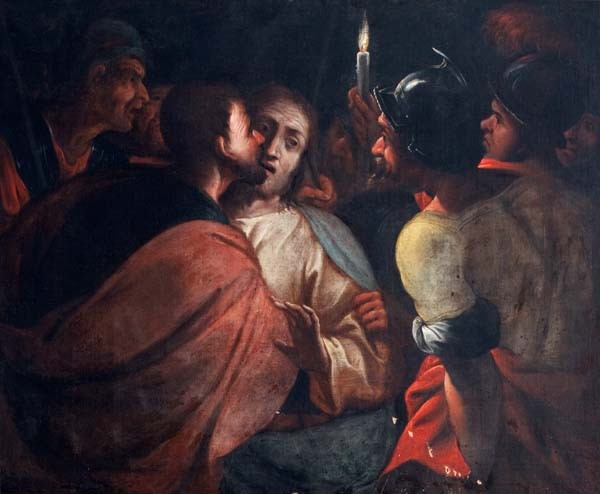
\includegraphics[width=0.48\textwidth]{nirp_caravaggio_1962_139_1}
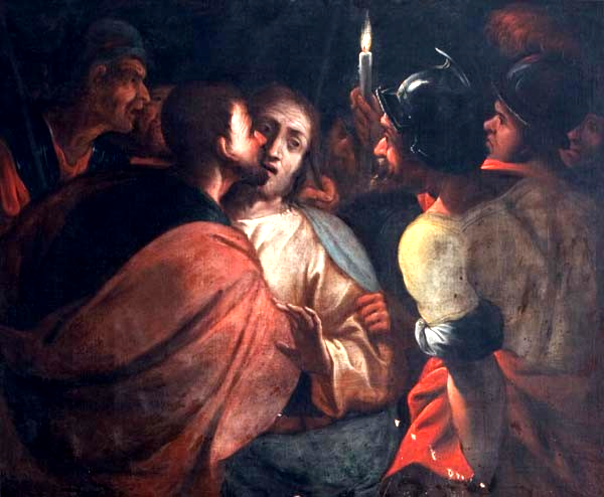
\includegraphics[width=0.48\textwidth]{caravaggio_1962_139_1}
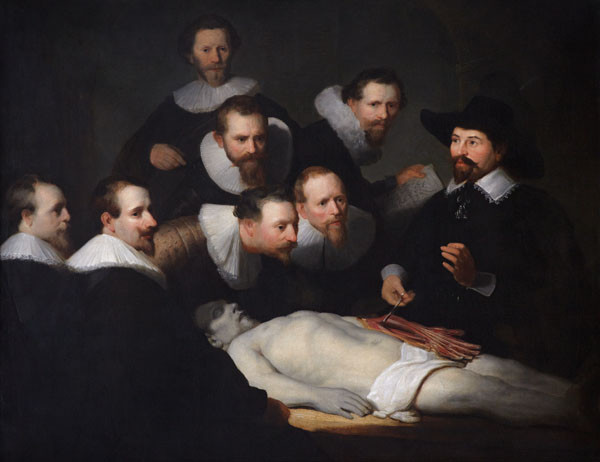
\includegraphics[width=0.48\textwidth]{nirp_rembrandt_eu_464}
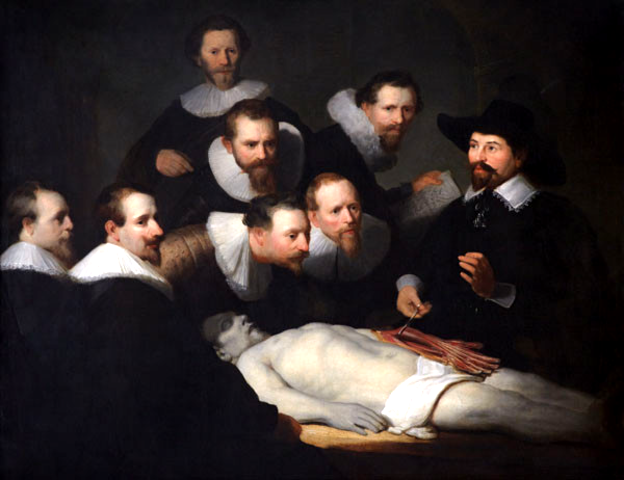
\includegraphics[width=0.48\textwidth]{rembrandt_eu_464}
\caption[Colour normalisation]{To the left are the original images, to the
right normalised ones.  It can be seen that the normalised images are brighter
to the human eye, this is because the darker and brighter colours are further
apart in the normalised images.  The top image is the "The Betrayal of Christ"
by \emph{Michelangelo da Caravaggio} and the image at the bottom is the "The
Anatomy Lesson of Dr. Nicolaes Tulp" by \emph{Rembranidt van Rijn}.}
\label{fig:norm}
\end{figure*}

As done by Romero and Machado in  \cite{jma12clas}, \emph{colour normalisation}
of the images is performed: for each channel, we subtract the minimum value
from all pixels, then divide all pixels by the value of the maximum value and
multiply by 255.  Different pictures of the same painting may have been taken
under different illumination, colour normalisation removes this complexity

\begin{figure*}[!htb]
\begin{equation}
\begin{aligned}
H_{HSV}  &= atan2\left(\frac{\sqrt{3}}{2}(G-B), \frac{1}{2}(2R-G-B)\right) \\
V_{HSV}  &= max(R,G,B) \\
S_{HSV}  &= \left\{
  \begin{array}{ll}
    0  &  \text{if } V = 0, \\
    \frac{\sqrt{ \left(\frac{\sqrt{3}}{2}(G-B)\right)^2
               + \left(\frac{1}{2}(2R-G-B)\right)^2 }}{V}
  &  \text{otherwise}. \\
  \end{array}
            \right.
\label{eq:hsv}
\end{aligned}
\end{equation}
\end{figure*}

\begin{figure*}[!htb]
\begin{equation}
\begin{aligned}
H_{HSL}  &= atan2\left(\frac{\sqrt{3}}{2}(G-B), \frac{1}{2}(2R-G-B)\right) \\
L_{HSL}  &= \frac{1}{2}max(R,G,B) + \frac{1}{2}min(R,G,B) \\
S_{HSL}  &= \left\{
  \begin{array}{ll}
    0  &  \text{if } L \in \{0,1\}, \\
    \frac{\sqrt{ \left(\frac{\sqrt{3}}{2}(G-B)\right)^2
               + \left(\frac{1}{2}(2R-G-B)\right)^2 }}{1 - \lvert 2L-1 \rvert}
  &  \text{otherwise}. \\
  \end{array}
           \right.
\label{eq:hsl}
\end{aligned}
\end{equation}
\end{figure*}

\begin{equation}
CS_{HSV} = \frac{S_{HSV} \times V_{HSV}}{255}
\label{eq:cs}
\end{equation}

The \emph{HSV colour space} was used by Romero \cite{jma12clas} in his work to
extract the features, on the other hand Machajdik \cite{mach10clas} uses the
\emph{HSL colour space} for the features in her work.  Both HSV and HSL colour
spaces are closer to how we humans perceive an image rather than the \emph{RGB
colour space}.  All images in the dataset are in RGB therefore we use
ImageMagick\footnote{ \href{http://imagemagick.org/}{http://imagemagick.org/} }
to convert the images into HSV and HSL colour spaces, the conversions are
depicted by Equation \ref{eq:hsv} and Equation \ref{eq:hsl}.  Each channel
(\emph{Hue}, \emph{Saturation}, \emph{Value} and \emph{Lightness}) is stored as
a Portable Graymap (PGM)\footnote{One of the \texttt{netpbm} formats for images
(PPM, PGM and PBM)}.  This format stores the channel uncompressed, which is
important for the calculation of the Kolmogorov complexity (one of the intended
features).  From the Equations \ref{eq:hsv} and \ref{eq:hsl} we can see that
the Hue is the same for both HSV and HSL colour spaces, yet the Saturation is
different.  We, therefore, store 5 channels (each as a separate PGM) for each
image: \emph{Hue}, \emph{Saturation$_{HSV}$}, \emph{Saturation$_{HSL}$},
\emph{Value}, and \emph{Lightness}.  Each channel is separated from the
original image as a single operation due to a limitation where ImageMagick
concatenates all channels into the output image when extracting three channels
at the same time.

In \cite{rmc12ajs} Romero defines an extra image channel from which he extracts
features, the \emph{colourfulness of the image}.  The colourfulness is the hue
of the image damped by the saturation, in the HSV colour space.  To achieve the
colourfulness the hue and saturation are multiplied and scaled to a range
between 0 and 255.  We developed a script (\texttt{sv2cs.py}) that performs the
calculation of the colourfulness of the image from the hues and saturation
according to the Equation \ref{eq:cs}.  Note that ImageMagick already scales
the hue channel to values between 0 and 255 when separating the channels,
therefore the Equation results in values in the range between 0 and 255.

Feature extractors then run on some or all of the six "channels" of the image:
\emph{Hue}, \emph{Saturation$_{HSV}$}, \emph{Saturation$_{HSL}$}, \emph{Value},
\emph{Lightness} and \emph{Colourfulness}.  Although these are not strictly
image channels, because the combination of them do not form the original image,
we will refer to these six representations as "image channels" throughout the
rest of the document for simplicity.

\begin{figure*}[tbp]
\centering
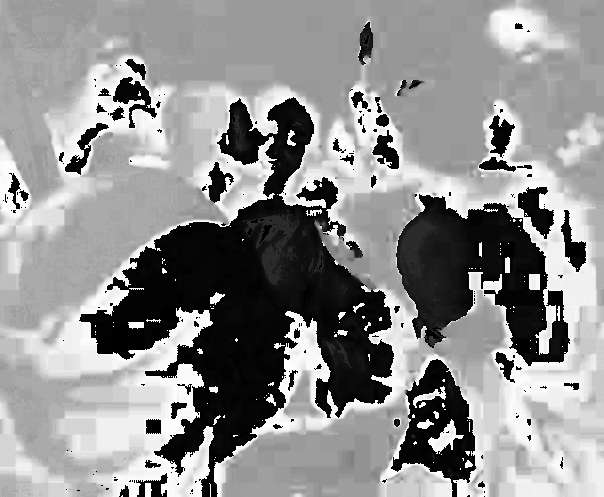
\includegraphics[width=0.30\textwidth]{H_caravaggio_1962_139_1}
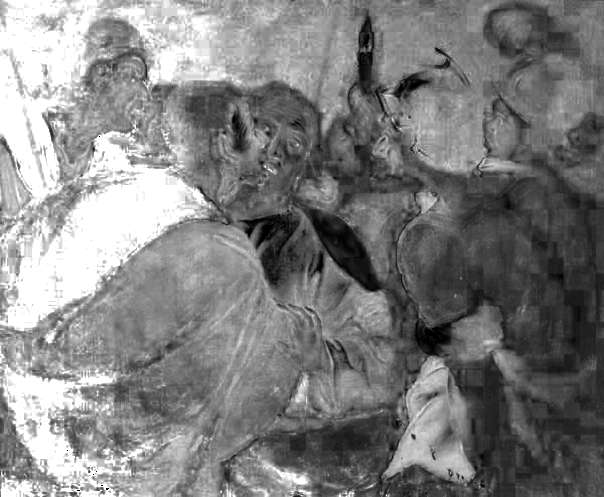
\includegraphics[width=0.30\textwidth]{SHSV_caravaggio_1962_139_1}
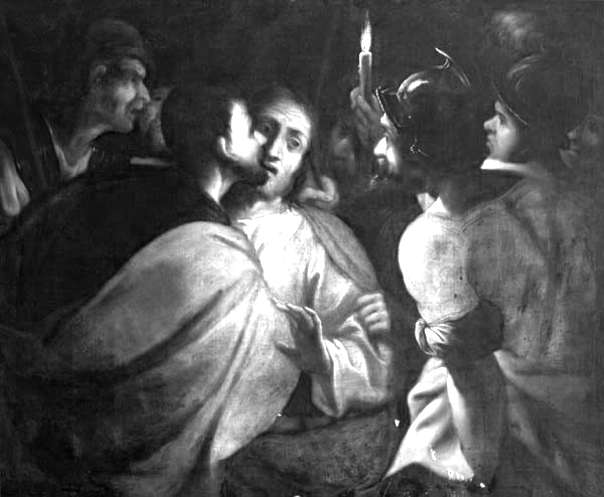
\includegraphics[width=0.30\textwidth]{V_caravaggio_1962_139_1}
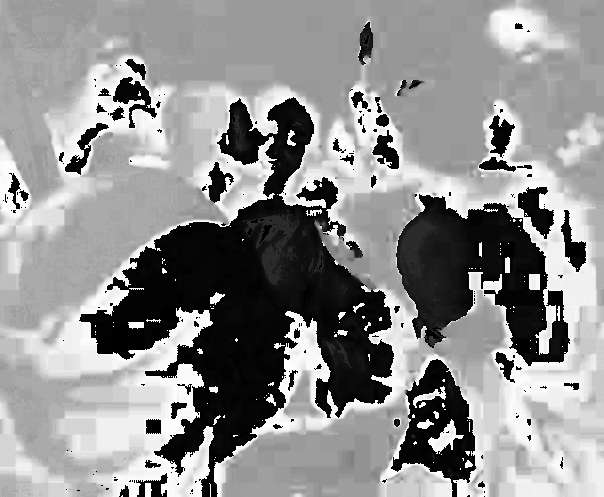
\includegraphics[width=0.30\textwidth]{H_caravaggio_1962_139_1}
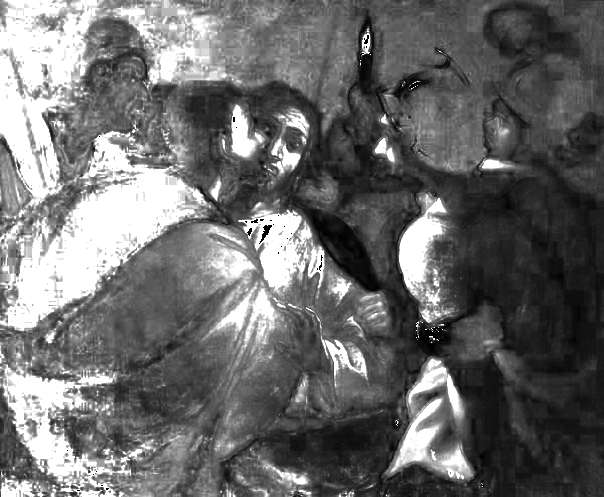
\includegraphics[width=0.30\textwidth]{SHSL_caravaggio_1962_139_1}
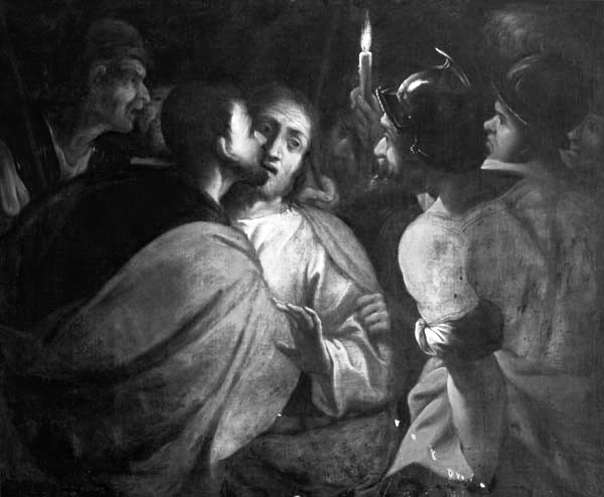
\includegraphics[width=0.30\textwidth]{L_caravaggio_1962_139_1}
\caption[HSV/HSL separation]{HSV/HSL separation of "The Betrayal of Christ".
At the top are the channels \emph{Hue}, \emph{Saturation} and \emph{Value} of
the HSV representation, at the bottom are the \emph{Hue}, \emph{Saturation} and
\emph{Lightness} channels of the HSL representation.  The \emph{Hue} channel is
the same in both representations, whilst the \emph{Saturation} and the third
channel is different across the representations.}
\label{fig:hsvl}
\end{figure*}

\begin{figure*}[tbp]
\centering
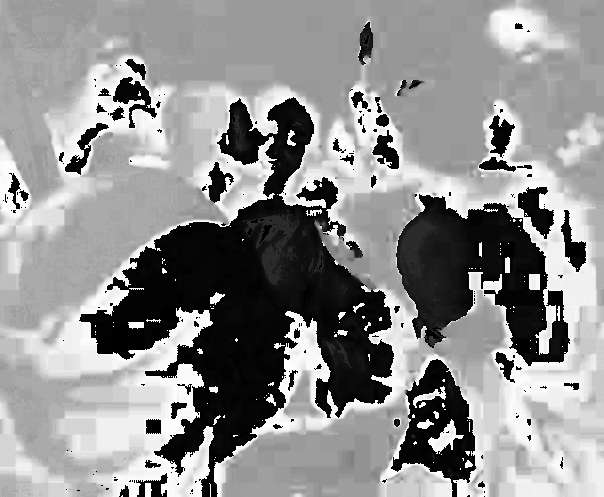
\includegraphics[width=0.30\textwidth]{H_caravaggio_1962_139_1}
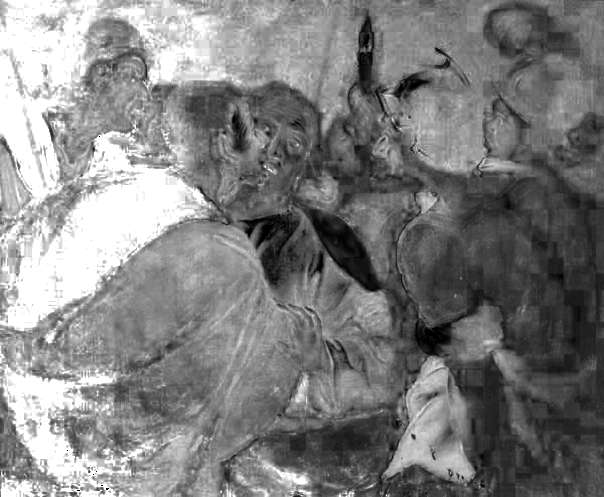
\includegraphics[width=0.30\textwidth]{SHSV_caravaggio_1962_139_1}
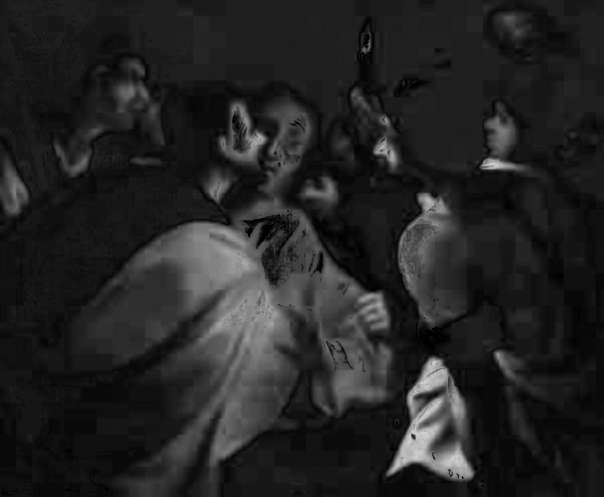
\includegraphics[width=0.30\textwidth]{CS_caravaggio_1962_139_1}
\caption[Colourfulness]{The \emph{Colourfulness} (right) of an image can be
derived from it's \emph{Hue} channel (left) and it's \emph{Saturation} channel
(centre), taken from the HSV representation.  Both channels are multiplied and
scaled as seen in equation \ref{eq:cs}.}
\label{fig:cs}
\end{figure*}

%Citations useful for the introduction (and for the remaining of the text too):
%Romero \cite{jma12clas}, Romero \cite{rmc12ajs}, Chen (Yahoo) on JSONS
%\cite{chen09yahoo}, Zirnhelt (generic artist classification)
%\cite{zirnhelt07art}, Machajdik (affective) \cite{mach10clas}, Chih-Wei
%(libsvm) \cite{hcl03svm}, DiMaggio (art classification) \cite{dimaggio87art}

\section{Basic Features}

Some features shall be retrieved from each of the six image channels.  From
Romero's work in \cite{rmc12ajs} we extract the features the are an
approximation of \emph{Kolmogorov complexity} of each of the channels; used in
Machajdik's work \cite{mach10clas} and Zirnhelt's work \cite{zirnhelt07art} the
features based on texture are calculated on the \emph{Grey Level Co-occurrence
Matrix} of each channel.  The \emph{average and standard deviation of all
pixels} in each of the channels is a common feature used across all three works
\cite{jma12clas,zirnhelt07art,mach10clas}.  Machajdik \cite{mach10clas} also
proposes to use the average and standard deviation of the pixels in the central
rectangle of the image when it is divided into three parts on it's width and
three parts on it's height, a \emph{Rule of thirds} of the image framing.

For each of these groups of features a feature extractor was built and run over
all images in the dataset.

\subsection{Kolmogorov complexity}

To estimate the Kolmogorov complexity of each channel we follow Romero's
procedure \cite{jma12clas} in finding the ratio between the file size of
uncompressed and compressed, using lossy compression, images.  The PGM format,
in which all channels of the image are stored, is an uncompressed format.  To
produce compressed images we use \emph{JPEG compression}, which is a lossy
compression format.

Following Romero in \cite{jma12clas} we produce the estimates of complexity not
only for each channel but for the edges that can be found in the channel.  We
use two edge detector filters: the \emph{Sobel} filter and the \emph{Canny}
filter, both provided by the \texttt{skimage.filter} python library.  For each
channel we produce a Sobel filtered uncompressed channel (in PGM format) and a
Canny filtered uncompressed channel (also in PGM format).  This totals for 18
PGM images for each image in the dataset.

Next, we compress each of the 18 images with JPEG compression with different
quality values.  We use the JPEG quality of 60, 40 and 20, following the same
quality values used by Romero \cite{jma12clas}.  This produces 3 JPEG images
for each of the 18 PGM images, giving a total of 54 JPEG compressed images for
each image in the dataset.

The Kolmogorov complexity is estimated by dividing the size (in bytes) of the
PGM image by each of it's correspondent JPEG compressed images.  This procedure
generates 54 features for each image in the dataset.

% We did not use any form of fractal compression.

\subsection{Grey Level Co-occurrence Matrix}

All features of texture coming from that.

For each channel we build three GLCMs, one using neighbouring pixels (next
pixel to the left), one using the next 6th pixel to the left and one using the
next 20th pixel to the left.  For each of these GLCM we calculate the contrast,
energy, homogeneity and correlation of the texture.  Correlation is not always
possible to calculate, in such cases we consider the texture correlation as 1.

\begin{figure*}[tbp]
\centering
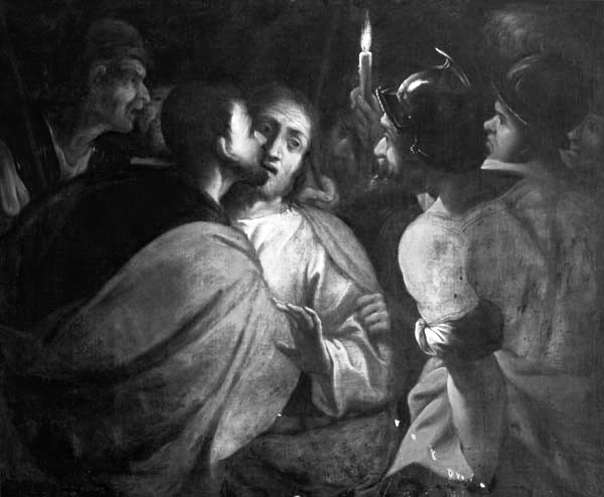
\includegraphics[width=0.30\textwidth]{L_caravaggio_1962_139_1}
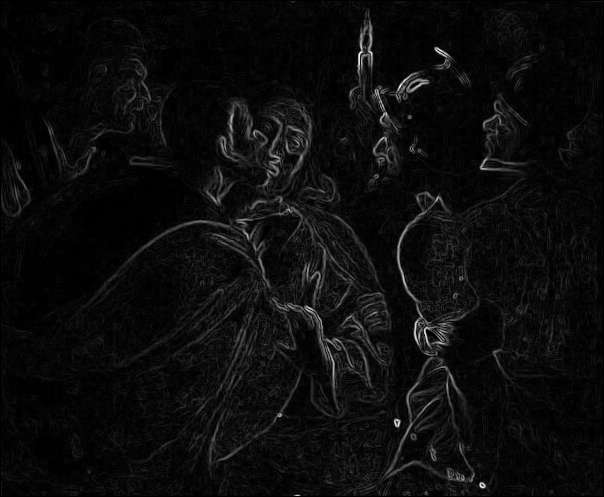
\includegraphics[width=0.30\textwidth]{sobel_L_caravaggio_1962_139_1}
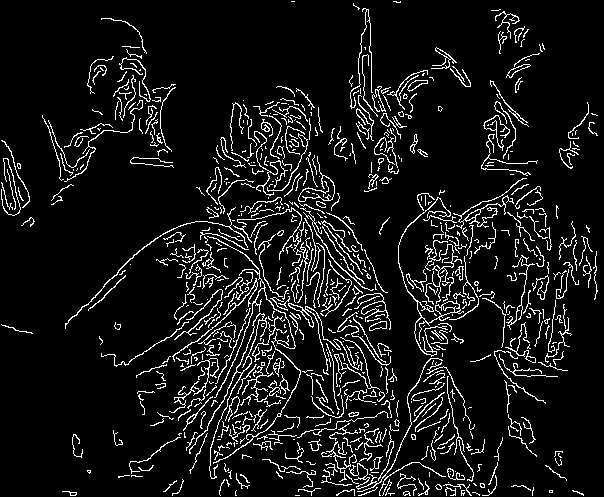
\includegraphics[width=0.30\textwidth]{canny_L_caravaggio_1962_139_1}
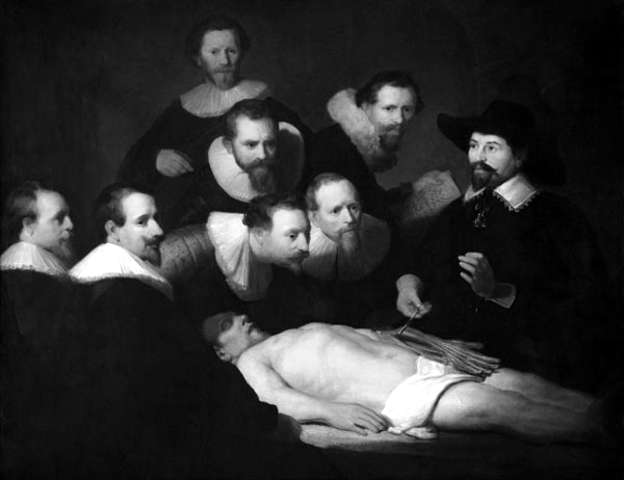
\includegraphics[width=0.30\textwidth]{L_rembrandt_eu_464}
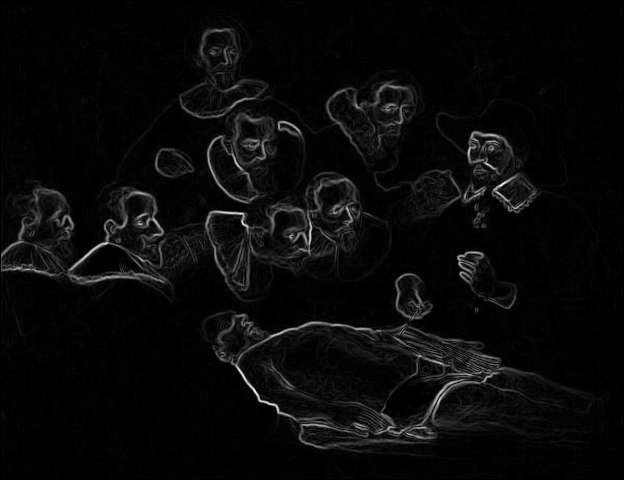
\includegraphics[width=0.30\textwidth]{sobel_L_rembrandt_eu_464}
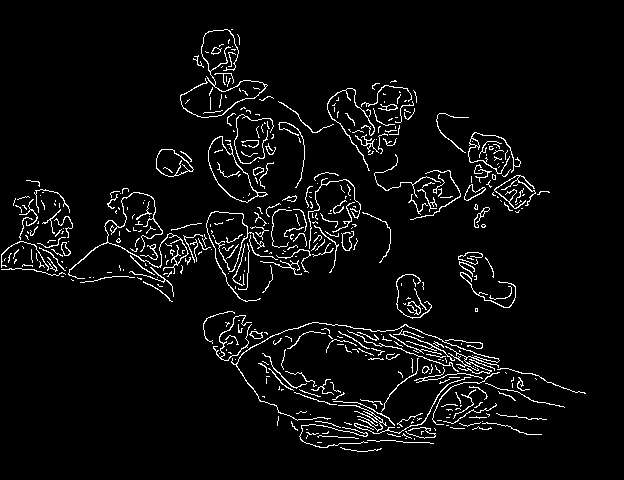
\includegraphics[width=0.30\textwidth]{canny_L_rembrandt_eu_464}
\caption[Canny and Sobel filters of Lightness]{Canny and Sobel filters of the
Lightness channel of an image.  For both images, to the left is the lightness
channel, in the centre is the \emph{Sobel filter} applied to this channel and
to the right is the \emph{Canny filter} applied to this channel.}
\label{fig:cannysobell}
\end{figure*}

\begin{figure*}[tbp]
\centering
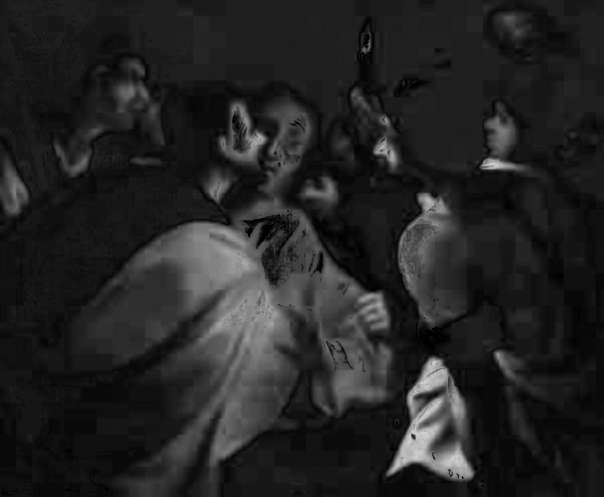
\includegraphics[width=0.30\textwidth]{CS_caravaggio_1962_139_1}
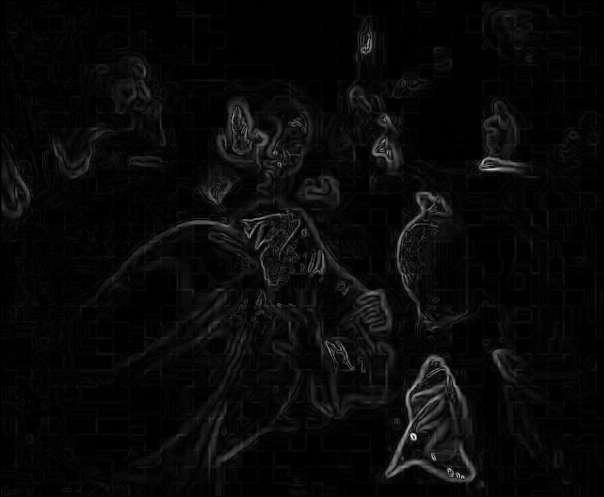
\includegraphics[width=0.30\textwidth]{sobel_CS_caravaggio_1962_139_1}
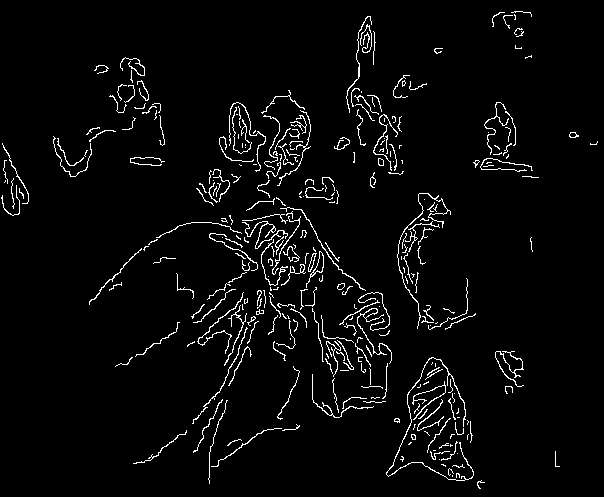
\includegraphics[width=0.30\textwidth]{canny_CS_caravaggio_1962_139_1}
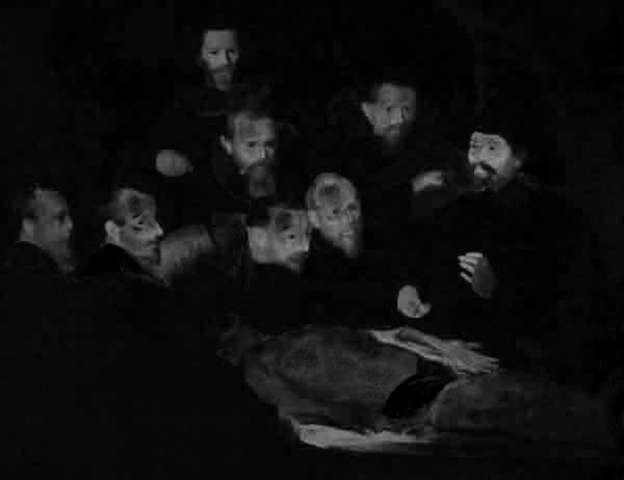
\includegraphics[width=0.30\textwidth]{CS_rembrandt_eu_464}
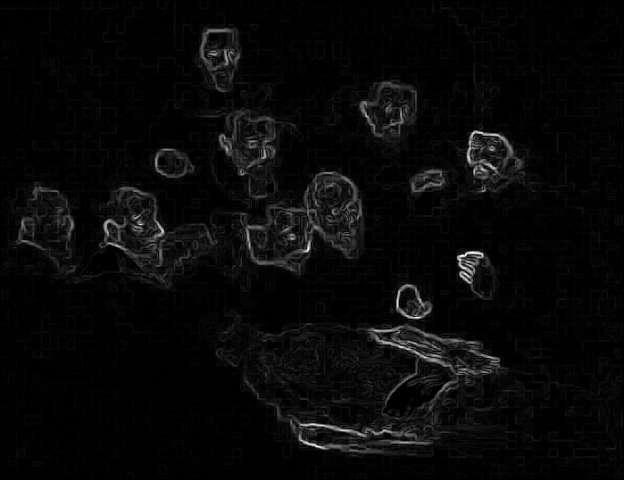
\includegraphics[width=0.30\textwidth]{sobel_CS_rembrandt_eu_464}
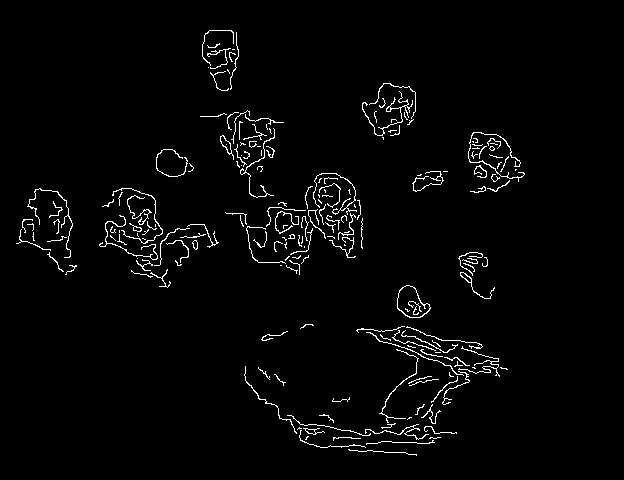
\includegraphics[width=0.30\textwidth]{canny_CS_rembrandt_eu_464}
\caption[Canny and Sobel filters of Colourfulness]{Canny and Sobel filters of
Colourfulness.  Again, to the left is the original image, in the centre the
\emph{Sobel filter} is applied and to the right the \emph{Canny filter} is
applied.}
\label{fig:cannysobelcs}
\end{figure*}

\subsection{Rule of Thirds}

Same averages on the central rectangle.

Average per channel, Standard deviation per channel on the central rectangle
only.

\subsection{Image Averages}

Std and average, super simple.

Average per channel, Standard deviation per channel.

\section{Itten Colours}

Stuff based on itten colours

\subsection{Amount of each colour}

Only the colours above the image average get counted.

Scale 0-255 into 0-360 and add 15 degrees to account for red being centered
at zero.  After this we have the following 12 bins:

\begin{verbatim}
red           (r)
orange red    (or)
orange        (o)
orange yellow (oy)
yellow        (y)
green yellow  (gy)
green         (g)
green blue    (gb)
blue          (b)
purple blue   (pb)
purple        (p)
purple red    (pr)
\end{verbatim}

Most prominent colours only.  All colours below the average of colours are
taken to be zero.

\subsection{Segmentation}

To measure contrasts we need to segment the image.  Rule of thirds, rule of
sevenths, watershed segmentation.

In rule of thirds and rule of sevenths we contrast all regions against all
other regions, but in the watershed segmentation we ignore the smallest
regions that are found.

\subsection{Itten Contrasts}

Contrast of hue, saturation, light and dark, warm and cold colours,
complements.

In watershed segmentation contrast only regions bigger than 548 pixels (square
root of 300 000)

\begin{figure*}[!htb]
\begin{equation}
\begin{aligned}
n_1       &= max(0.1, 1 - warm_1 - cold_1) \\
n_2       &= max(0.1, 1 - warm_2 - cold_2) \\
contrast  &= \frac{ max\left( \left\lvert \frac{warm_1}{warm_2}
                                        - \frac{cold_1}{cold_2} \right\rvert
                            , \left\lvert \frac{warm_2}{warm_1}
                                        - \frac{cold_2}{cold_1} \right\rvert
                       \right)
                 }{ n_1 \times n_2 }
\label{eq:coldwarm}
\end{aligned}
\end{equation}
\end{figure*}

\begin{figure*}[!htb]
\begin{equation}
\begin{aligned}
n_1       &= 1 - warm_1 - cold_1 \\
n_2       &= 1 - warm_2 - cold_2 \\
contrast  &= \frac{ warm_1 \times warm_2
                   + n_1    \times n_2
                   + cold_1 \times cold_2
                  }{ \sqrt{      (warm_1^2 + n_1^2 + cold_1^2)
                          \times (warm_2^2 + n_2^2 + cold_2^2) } }
\label{eq:mach}
\end{aligned}
\end{equation}
\end{figure*}

\begin{figure*}[!htb]
\begin{equation}
D = min( \lvert H_1 - H_2 \rvert , 360 - \lvert H_1 - H_2 \rvert )
\label{eq:wheel}
\end{equation}
\end{figure*}

Warm and cold contrast is represented by the value of warm colours, cold
colours and a value of neutrality which is 1 minus the scaled amount of warm
and cold colours.

\begin{verbatim}
red           (r)  --\
orange red    (or)   |  warm
orange        (o)    | colours
orange yellow (oy) --/
yellow        (y)
green yellow  (gy)
green         (g)  --\
green blue    (gb)   |  cold
blue          (b)    | colours
purple blue   (pb) --/
purple        (p)
purple red    (pr)
\end{verbatim}

% We did not do the contrast of extension, as it was not described.  Also we
% did not perform the Itten Harmony as it is the absence of contrast of
% complements.

The contrast is: the average of the region scaled by the size of the region and
then contrasted against all other regions.  We then take the biggest contrast
value from all contrasts (not in contrast of hue and complements when watershed
segmentation is used, in this case we use another technique).  Calculating the
contrast value is done in many ways: warm vs cold, complements of colours,
saturation, lightness or value.

Contrast of saturation x2 (HSV and HSL)

Contrast of light and dark x2 (Lightness and value)

Contrast of Hue x2 (Hue and Colourfulness)

Contrast of Complements x2 (Hue and Colourfulness) here we also consider only
the most prominent hues.  Hues amounting for less than 5\% of colours are
ignored.

When contrast of hue or of complements is done over the watershed segmented
image we take the number of high contrasts (two regions that have a high
contrast between themselves).  For the contrast on the hue channel we count a
contrast each time we find two regions with a contrast of more than 160 degrees
(remember it's a circle), and for the contrast on the colourfulness channel we
count a contrast for every two regions with more than 125 degrees (because the
contrast is damped by the saturation).

The equation for contrast of cold and warm in Machajidik's work \ref{eq:mach}
represents well contrasts when the amount of cold and warm colours varies
across the regions we calculate the contrast.  Yet Machajidik's equation
performs a poor estimate when one region is completely warm and another region
completely cold, in this case the equation results in a contrast value smaller
than if the regions had less warmth and coldness.  To work around this issue we
developed another equation for the cold and warm contrast \ref{eq:coldwarm}.
The contrast by this equation scales up when one region is highly warm and the
other highly cold, also there is a hard limit for the neutrality of a region
which cannot be come less than 0.1.

\begin{figure*}[tbp]
\centering
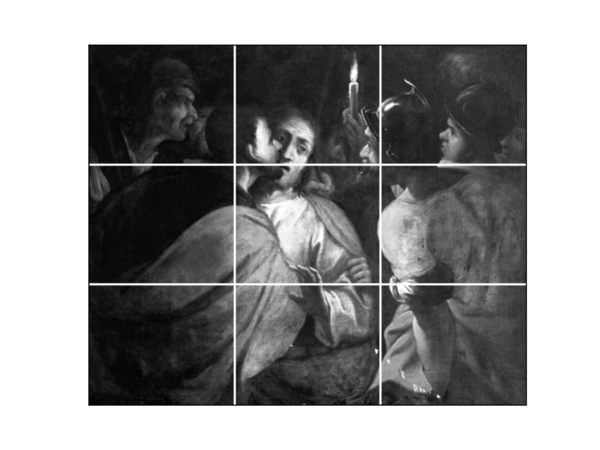
\includegraphics[width=0.48\textwidth]{r3_L_caravaggio_1962_139_1}
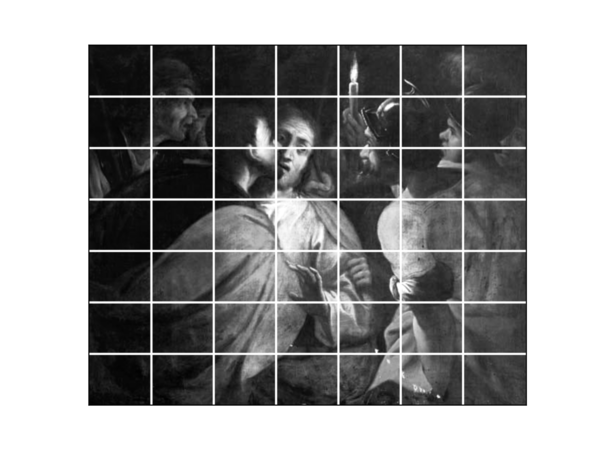
\includegraphics[width=0.48\textwidth]{r7_L_caravaggio_1962_139_1}
\caption[Rule of thirds]{Rule of \emph{thirds} consist of dividing the image
into three equal parts on each axis, as seen on the image on the left.  It is
common that the colours and objects in the central region are the most
important for the scene painted.  A rule of \emph{sevenths}, figure on the
right, was also used in the segmentation process.  Dividing into seven equal
parts on each axis produce smaller regions than the rule of thirds but big
enough to be noticeable for the contrast of the image.}
\label{fig:r3}
\end{figure*}

\begin{sidewaysfigure*}[p]
\centering
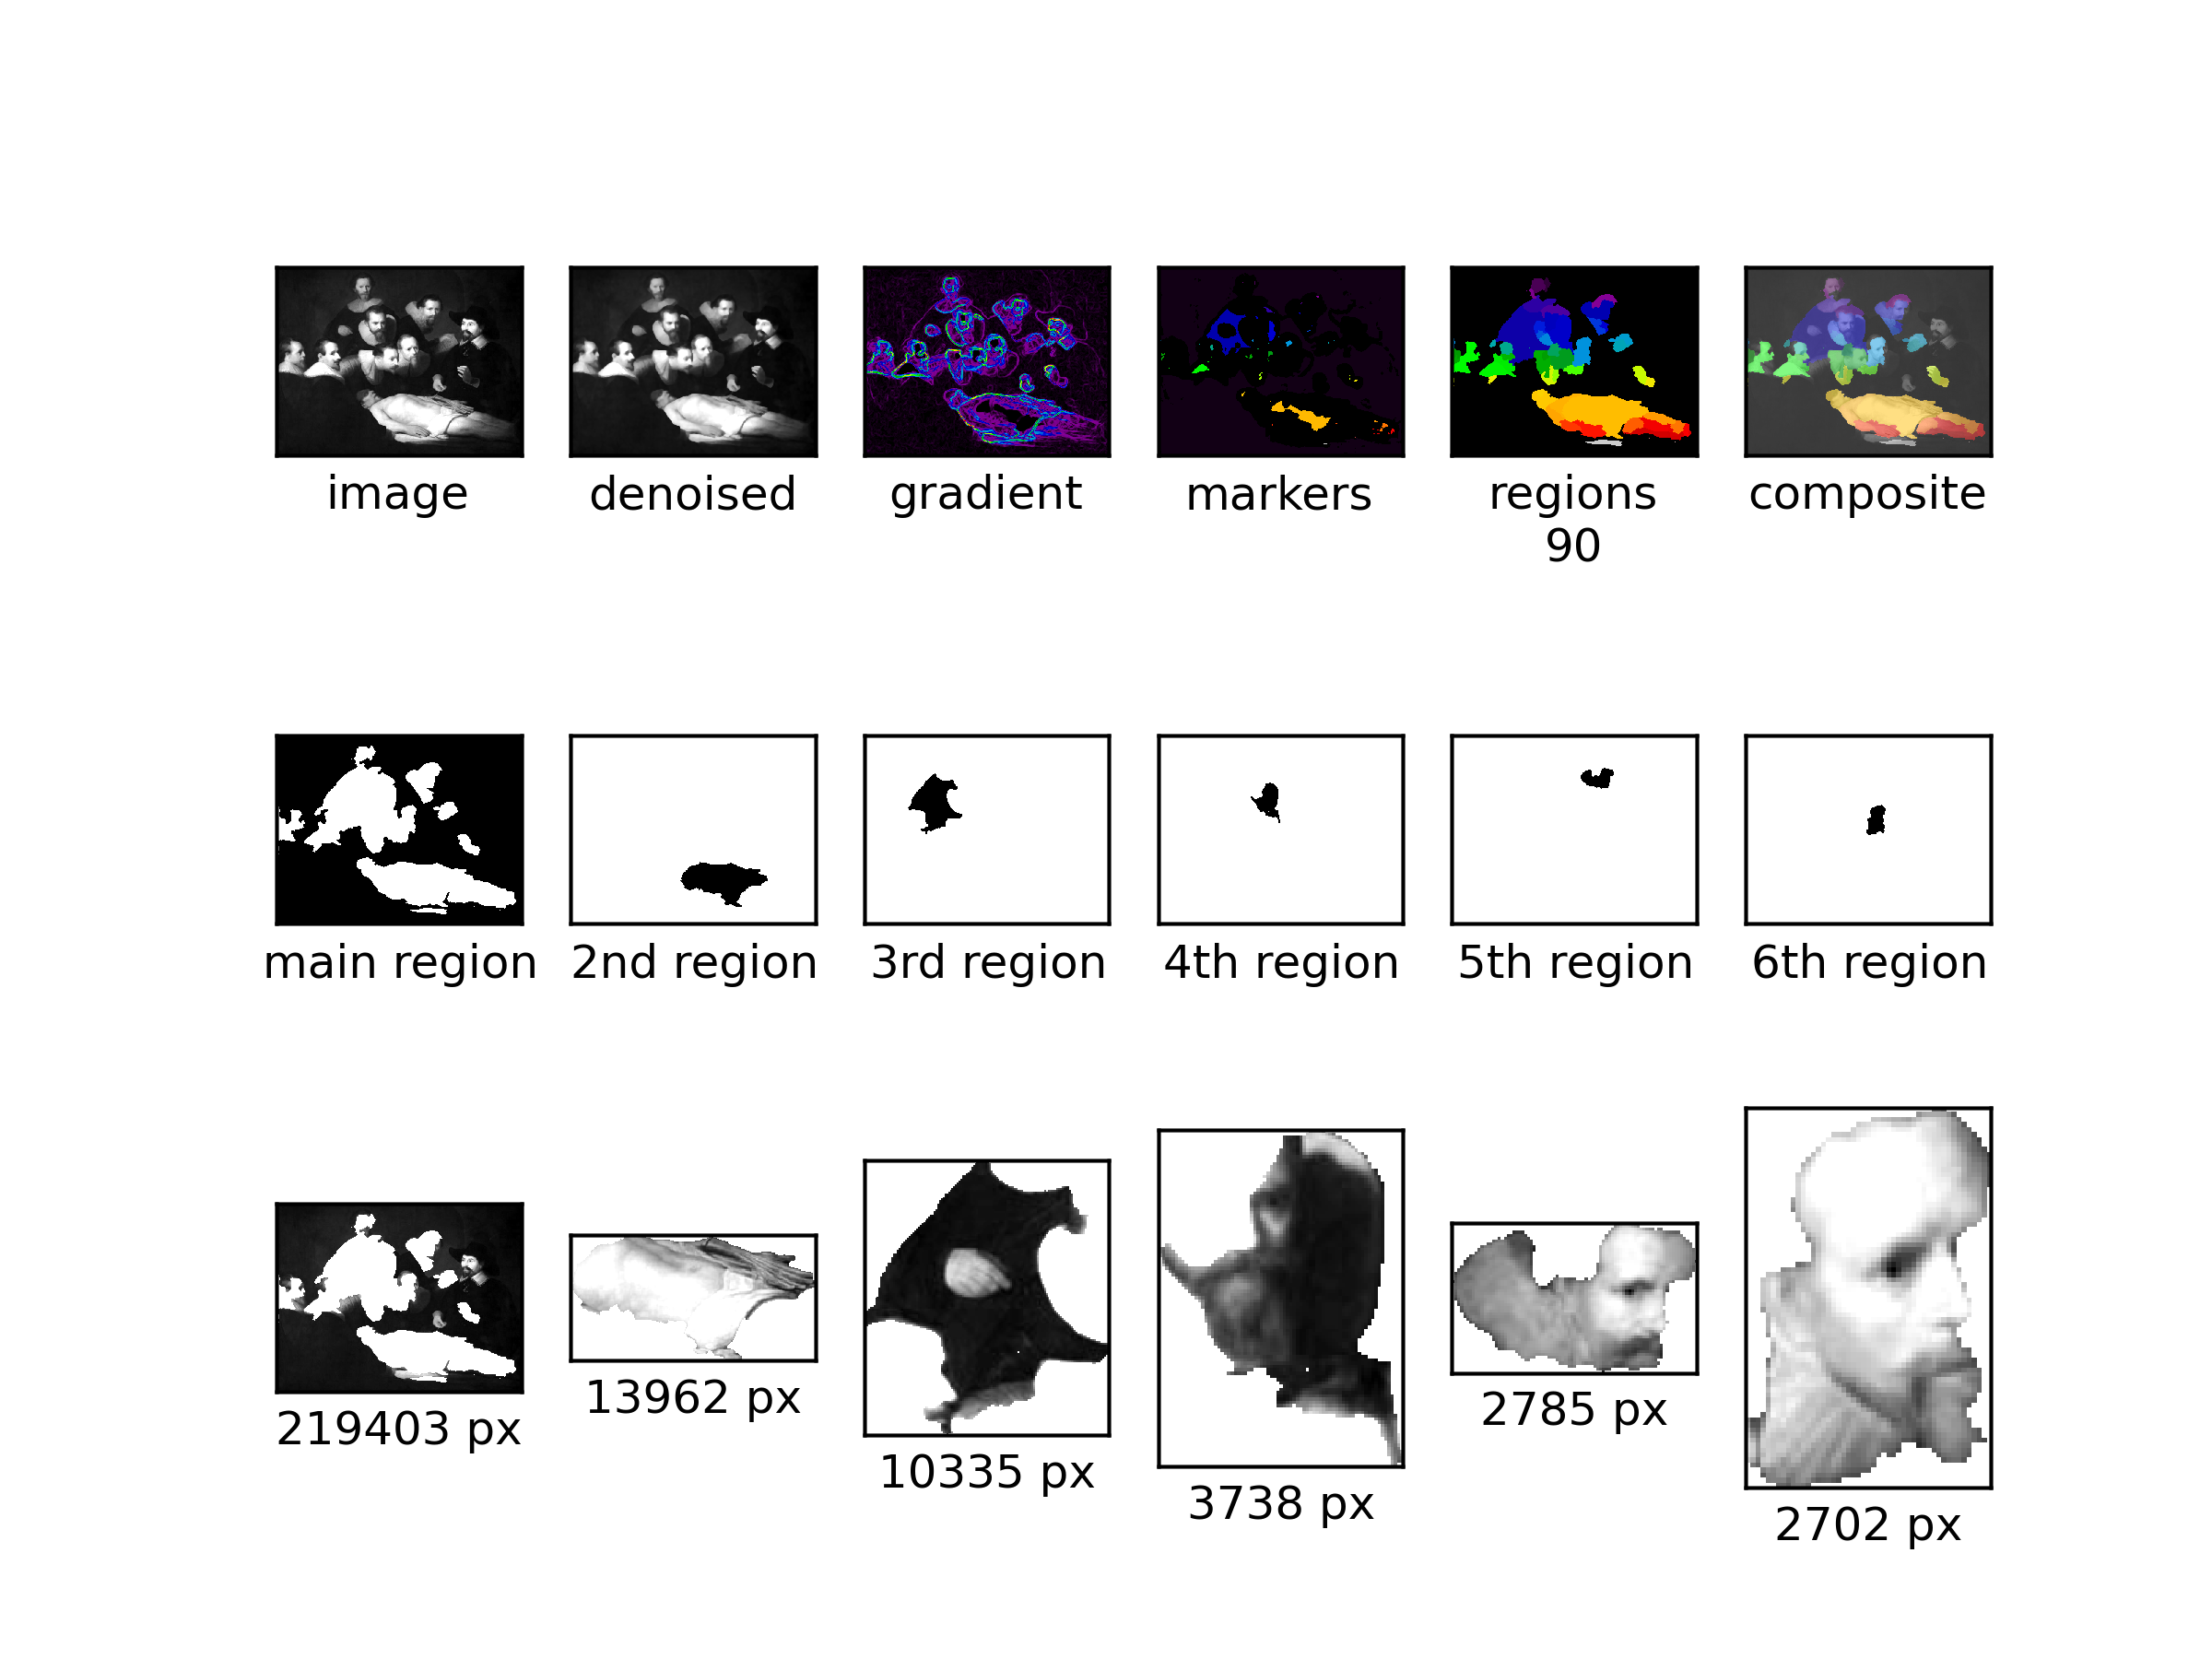
\includegraphics[width=0.9\textwidth]{segm_rembrandt_eu_464}
\caption[Watershed segmentation example]{Watershed segmentation example.  The
images at the top show the steps for the segmentation of the image.  The
original image, a denoised image on which the segmentation is actually made,
the gradient magnitude, and the original places of the markers.  Next the
markers \emph{flow as water} filling the regions, this is shown on the next
image.  Finally, the last image in the first row shows how the found regions
are distributed over the original image.  The second row show the five biggest
regions found as a mask over the image.  The last row show the mask generated
by each of the five biggest regions applied to the image and cropped.}
\label{fig:segm}
\end{sidewaysfigure*}

\section{Extra Metadata}

It was needed to classify the artists into art movements, some of this data
could be found on the museum website yet most of it needed to be evaluated by
hand.  The life period and country where the artist worked were the most
important points to classify him into an art movement.

\end{multicols}

\chapter{Results}
\label{chap:results}

% No PCA was done, we can say that the features are unrelated enough that we do
% not need feature selection.

% Pearson coefficient was not used, we do not have any categorical data instead
% all data for correlation is numeric.

% Extrapolation towards, art movement/school is the most important part of this
% chapter.

\begin{multicols}{2}

\section{Correlation between features}

Artists in the same art movement shall be close, in distinct movements shall be
apart.

The absolute value of the correlation coefficient on the scatter graph shall be
good enough.  It can be seen on the graph that few correlation coefficients are
above 0.7.

\section{Classification}

How we calculated the correlation.  Most significant numbers from each table.
A plethora of tables.  A graph with three most prominent features between each
school.

\begin{table*}[htp]  % table* instead of table because of multicols
\centering
\begin{tabular}{|l|l|}
\toprule
Art Movement & Artists (number of paintings) \\
\bottomrule \toprule
\multirow{2}{*}{Renaissance (126)}
                     &  Bassano (17), Botticelli (6), Raphael (52), \\
                     &  Titian (34), Veronese (17)                  \\
\midrule
\multirow{7}{*}{Baroque (521)}
                     &  Berchem (47), Caravaggio (8), Cuyp (20),      \\
                     &  Dujardin (14), Greco (4), Hondecoeter (10),   \\
                     &  Miereveld (12), Molenaer (12), Monnoyer (19), \\
                     &  Murillo (38), Poussin (20), Rebecca (14),     \\
                     &  Rembrandt (30), Ribera (28), Ricci (25),      \\
                     &  Rosa (31), Rubens (61), Teniers (76),         \\
                     &  Vel\'azquez (24), Wouwerman (28)              \\
\midrule
\multirow{2}{*}{Neoclassicism (195)}
                     &  Canaletto (34), Carlevariis (51), Dughet (30), \\
                     &  Kauffmann (22), Panini (38), Zoffany (20)      \\
\midrule
\multirow{5}{*}{Romanticism (215)}
                     &  Boudin (26), Constable (39), Daubigny (13),  \\
                     &  Delacroix (9), Diaz (17), Gainsborough (13), \\
                     &  Goya (8), Latour (31), Leslie (10),          \\
                     &  Loutherbourg (17), Mulready (10),            \\
                     &  Rousseau (12),  Watts (10)                   \\
\midrule
Impressionism (32)   &  Gauguin (4), Monticelli (18), Pissarro (10) \\
\bottomrule \toprule
Watercolour (16)     &  Carpenter (9), Tagore (7) \\
\midrule
\multirow{2}{*}{Mughal (79)}
                     &  Basawan (11), Jagan (9), Kesav (15), La'l (19), \\
                     &  Miskin (15), Tulsi (10)                         \\
\midrule
N/A                  &  Devi (16) \\
\bottomrule
\end{tabular}
\caption[Artists in art movements]{Artists in art movements, or art schools.
Several simplifications were made to allow for a smaller number of classes.
The top of the table represents a simplified version of the \emph{history of
art in Europe}, starting with \emph{Renaissance} in the 15th-16th centuries,
\emph{Baroque} in the 17th century, \emph{Neoclassicism} in the 18th century,
\emph{Romanticism} containing all styles of the early 19th century and
\emph{Impressionism} including all styles of the late 19th century.  The bottom
of the table includes movements unrelated to the mentioned ones (\emph{Mughal
miniature painting style}) or using different materials (\emph{Watercolour}).}
\label{tab:style}
\end{table*}

nanan nanan nanan nanan nanan nanan nanan nanan nanan nanan nanan nanan nanan
nanan nanan nanan nanan nanan nanan nanan nanan nanan nanan nanan nanan nanan
nanan nanan nanan nanan nanan nanan nanan nanan nanan nanan nanan nanan nanan
nanan nanan nanan nanan nanan nanan nanan nanan nanan nanan nanan nanan nanan
nanan nanan nanan nanan nanan nanan nanan nanan nanan nanan nanan nanan nanan
batman

%\section{meeting: discussion on CBIR (Friday, 1st of July)}
%
%Amount of noise (by random sample) in the cleansed datasets.
%
%Start writing about dataset cleansing heuristics, plus some *descriptions* and
%*statistics*.
%
%Get some of the artists (with most paintings) and do some statistics over
%those.
%
%Histograms of features (especially itten colours) by different artists.
%
%R library to explore data: ggplot2 (use it?).
%
%%%%%%%%%%%%
% Features %
%%%%%%%%%%%%

% Kolmogorov complexity (quality at: 60, 40, 20)
%   JPEG compression: OK!
%   Fractal compression: DON'T BOTHER

% Itten colours
%   saturation, light and dark, extension, complement,
%   hue, warm and cold and simultaneous contrast:       OK!
%
%   harmony: OK!

% Texture (GLCM): OK!
% Edges (sobel and canny filters): OK!
% Rule of thirds: OK!

%%%%%%%%%%%%%%
% Evaluation %
%%%%%%%%%%%%%%

% PCA between pairs of authors
% Pearson correlation coefficient between pairs of authors

%%%%%%%%%%%%%%%%%
% Extrapolation %
%%%%%%%%%%%%%%%%%

% art period/school/movement classification


%nofilter-cs60 nofilter-cs40 nofilter-cs20 nofilter-h60 nofilter-h40
%nofilter-h20 nofilter-l60 nofilter-l40 nofilter-l20 nofilter-shsv60
%nofilter-shsv40 nofilter-shsv20 nofilter-shsl60 nofilter-shsl40 nofilter-shsl20
%nofilter-v60 nofilter-v40 nofilter-v20 sobel-cs60 sobel-cs40 sobel-cs20
%sobel-h60 sobel-h40 sobel-h20 sobel-l60 sobel-l40 sobel-l20 sobel-shsv60
%sobel-shsv40 sobel-shsv20 sobel-shsl60 sobel-shsl40 sobel-shsl20 sobel-v60
%sobel-v40 sobel-v20 canny-cs60 canny-cs40 canny-cs20 canny-h60 canny-h40
%canny-h20 canny-l60 canny-l40 canny-l20 canny-shsv60 canny-shsv40 canny-shsv20
%canny-shsl60 canny-shsl40 canny-shsl20 canny-v60 canny-v40 canny-v20

%\begin{sidewaystable*}[ptb]
%\begin{table*}[ptb]
%\centering
%\begin{tabular}{l|ccccccccc|}
%\large{\bf Correlation on Hue}
%  & \rotatebox{270}{Kolmogorov raw 60}
%  & \rotatebox{270}{Kolmogorov raw 40}
%  & \rotatebox{270}{Kolmogorov raw 20}
%  & \rotatebox{270}{Kolmogorov Sobel 60}
%  & \rotatebox{270}{Kolmogorov Sobel 60}
%  & \rotatebox{270}{Kolmogorov Sobel 40}
%  & \rotatebox{270}{Kolmogorov Canny 20}
%  & \rotatebox{270}{Kolmogorov Canny 40}
%  & \rotatebox{270}{Kolmogorov Canny 20}
%  \\
%\hline
%Kolmogorov raw 60  &1.01&2.01&3.01&4.01&5.01&6.01&7.01&8.01&9.01\\
%Kolmogorov raw 40  &    &2.01&3.01&4.01&5.01&6.01&7.01&8.01&9.01\\
%Kolmogorov raw 20  &    &    &3.01&4.01&5.01&6.01&7.01&8.01&9.01\\
%Kolmogorov Sobel 60&    &    &    &4.01&5.01&6.01&7.01&8.01&9.01\\
%Kolmogorov Sobel 40&    &    &    &    &5.01&6.01&7.01&8.01&9.01\\
%Kolmogorov Sobel 20&    &    &    &    &    &6.01&7.01&8.01&9.01\\
%Kolmogorov Canny 60&    &    &    &    &    &    &7.01&8.01&9.01\\
%Kolmogorov Canny 40&    &    &    &    &    &    &    &8.01&9.01\\
%Kolmogorov Canny 20&    &    &    &    &    &    &    &    &9.01\\
%\hline
%\end{tabular}
%\caption{Artists in art movements}
%\label{tab:corrstuff}
%\end{sidewaystable*}
%\end{table*}

\begin{table*}[ptb]
\centering
\rowcolors{1}{}{lightgray}
\begin{tabular}{|l|r||l|r||l|r|}
\toprule
artist & acc. & artist & acc. & artist & acc. \\
\midrule
basawan      &  54.55 & goya         &  87.50 & poussin      &  70.00 \\
bassano      &  76.47 & greco        & 100.00 & raphael      &  94.23 \\
berchem      &  85.11 & hondecoeter  &  80.00 & rebecca      &  92.86 \\
botticelli   & 100.00 & jagan        &  55.56 & rembrandt    &  80.00 \\
boudin       &  96.15 & kauffmann    &  68.18 & ribera       &  78.57 \\
canaletto    & 100.00 & kesav        &  86.67 & ricci        &  68.00 \\
caravaggio   &  87.50 & lal          &  89.47 & rosa         &  70.97 \\
carlevariis  & 100.00 & latour       &  87.10 & rousseau     &  66.67 \\
carpenter    & 100.00 & leslie       & 100.00 & rubens       &  88.52 \\
constable    & 100.00 & loutherbourg &  64.71 & tagore       & 100.00 \\
cuyp         &  85.00 & miereveld    & 100.00 & teniers      &  89.47 \\
daubigny     & 100.00 & miskin       &  60.00 & titian       &  79.41 \\
delacroix    &  66.67 & molenaer     &  66.67 & tulsi        &  50.00 \\
devi         & 100.00 & monnoyer     &  89.47 & velazquez    &  58.33 \\
diaz         &  88.24 & monticelli   &  88.89 & veronese     &  82.35 \\
dughet       &  80.00 & mulready     &  90.00 & watts        &  90.00 \\
dujardin     &  64.29 & murillo      &  92.11 & wouwerman    &  85.71 \\
gainsborough &  92.31 & panini       &  92.11 & zoffany      &  75.00 \\
gauguin      & 100.00 & pissarro     & 100.00 &              &        \\

\bottomrule
\end{tabular}
\caption[Multiclass artist classification]{Multiclass artist classification}
\label{tab:predart}
\end{table*}

\begin{table*}[ptb]
\centering
\begin{tabular}{|l|r||l|r|}
\toprule
school & acc. & school & acc. \\
\midrule
renaissance   &  50.00 & romanticism   &  65.12 \\
baroque       &  95.20 & impressionism &  71.88 \\
neoclassicism &  48.21 & mughal        & 100.00 \\

\bottomrule
\end{tabular}
\caption[Multiclass school classification]{Multiclass school classification}
\label{tab:predsch}
\end{table*}

\section{Cross Classification}

When we take two classes only and run the classifiers between them the results
are better.  This is because classification between two classes is easier as
classifiers can concentrate on specific points that are different between those
two classes.

nanan nanan nanan nanan nanan nanan nanan nanan nanan nanan nanan nanan nanan
nanan nanan nanan nanan nanan nanan nanan nanan nanan nanan nanan nanan nanan
nanan nanan nanan nanan nanan nanan nanan nanan nanan nanan nanan nanan nanan
nanan nanan nanan nanan nanan nanan nanan nanan nanan nanan nanan nanan nanan
nanan nanan nanan nanan nanan nanan nanan nanan nanan nanan nanan nanan nanan
batman

\begin{table*}[ptb]
\centering
\begin{tabular}{r||r|r|r|r|r}
\toprule
artist & titian & murillo & rembrandt & canaletto & constable \\
\midrule
murillo       &  72.22 &        &        &        &        \\
rembrandt     &  70.31 &  66.18 &        &        &        \\
canaletto     &  97.06 &  97.22 &  96.88 &        &        \\
constable     &  95.89 &  96.10 &  91.30 &  93.15 &        \\
monticelli    &  90.38 &  89.29 &  83.33 &  90.38 &  89.47 \\

\bottomrule
\end{tabular}
\caption[Two class artist classification]{Two class artist classification}
\label{tab:foldart}
\end{table*}

\begin{table*}[ptb]
\centering
\rowcolors{5}{}{lightgray}
\begin{tabular}{r||r|r|r|r|r}
\toprule
school & renaiss. & baroque & neoclass. & romantic. & impression. \\
\midrule
baroque       &  84.39 &        &        &        &        \\
neoclassicism &  82.87 &  80.03 &        &        &        \\
romanticism   &  84.46 &  79.21 &  77.07 &        &        \\
impressionism &  91.14 &  95.12 &  91.63 &  88.26 &        \\
mughal        & 100.00 & 100.00 & 100.00 & 100.00 & 100.00 \\

\bottomrule
\end{tabular}
\caption[Two class school classification]{Two class school classification}
\label{tab:foldsch}
\end{table*}

\begin{figure*}[tbp]
\centering
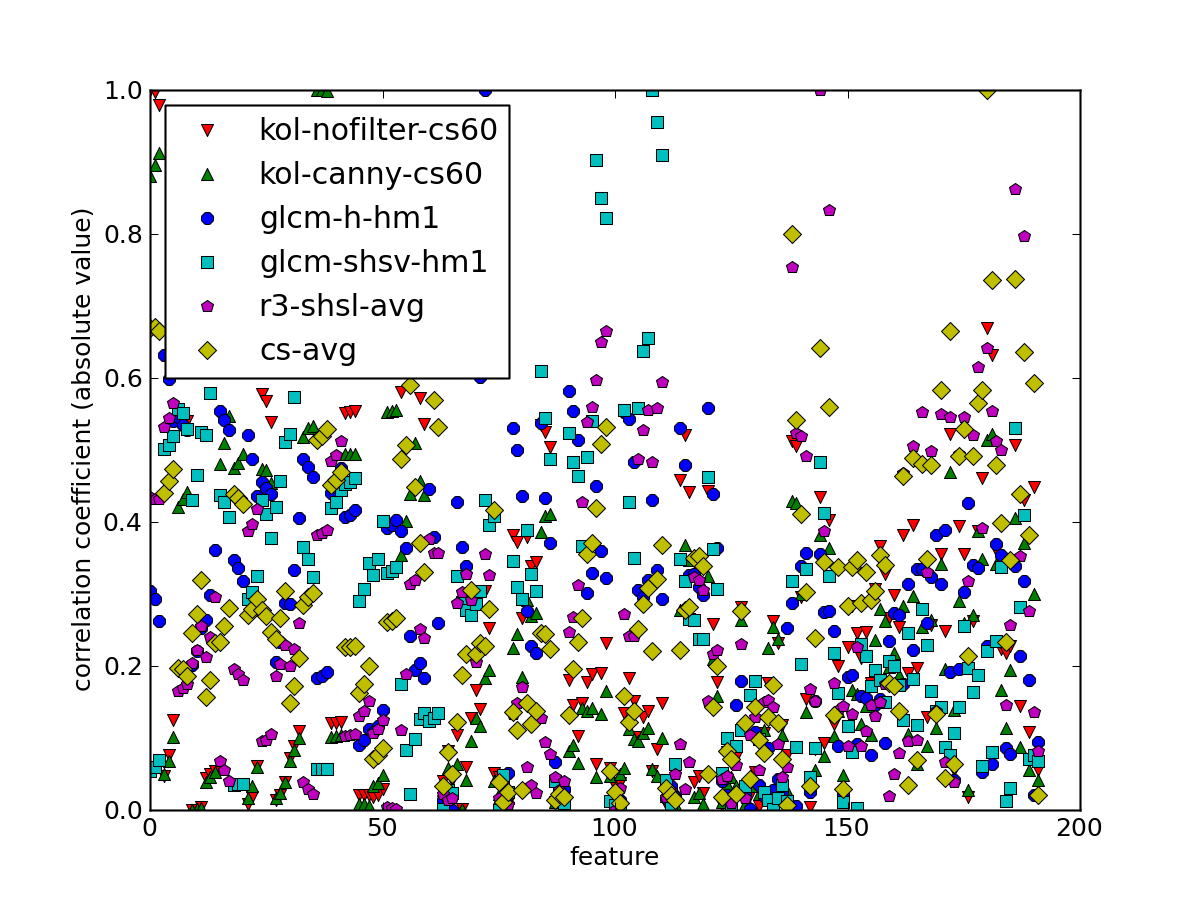
\includegraphics[width=\textwidth]{corr-graph}
\caption[Correlation]{Correlation Coefficient}
\label{fig:corr}
\end{figure*}

\begin{figure*}[tbp]
\centering
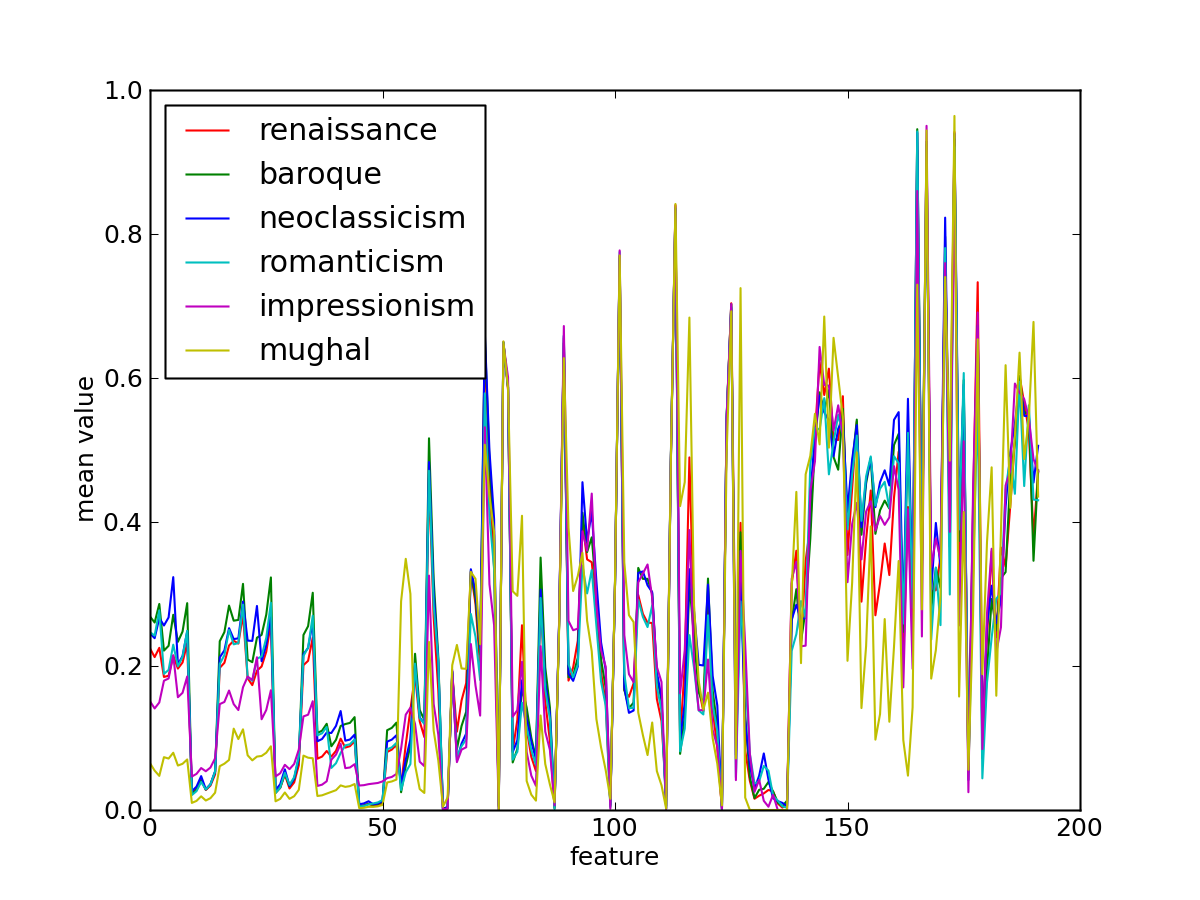
\includegraphics[width=\textwidth]{school-graph}
\caption[Feature Values]{Feature values per School}
\label{fig:school}
\end{figure*}

\begin{figure*}[tbp]
\centering
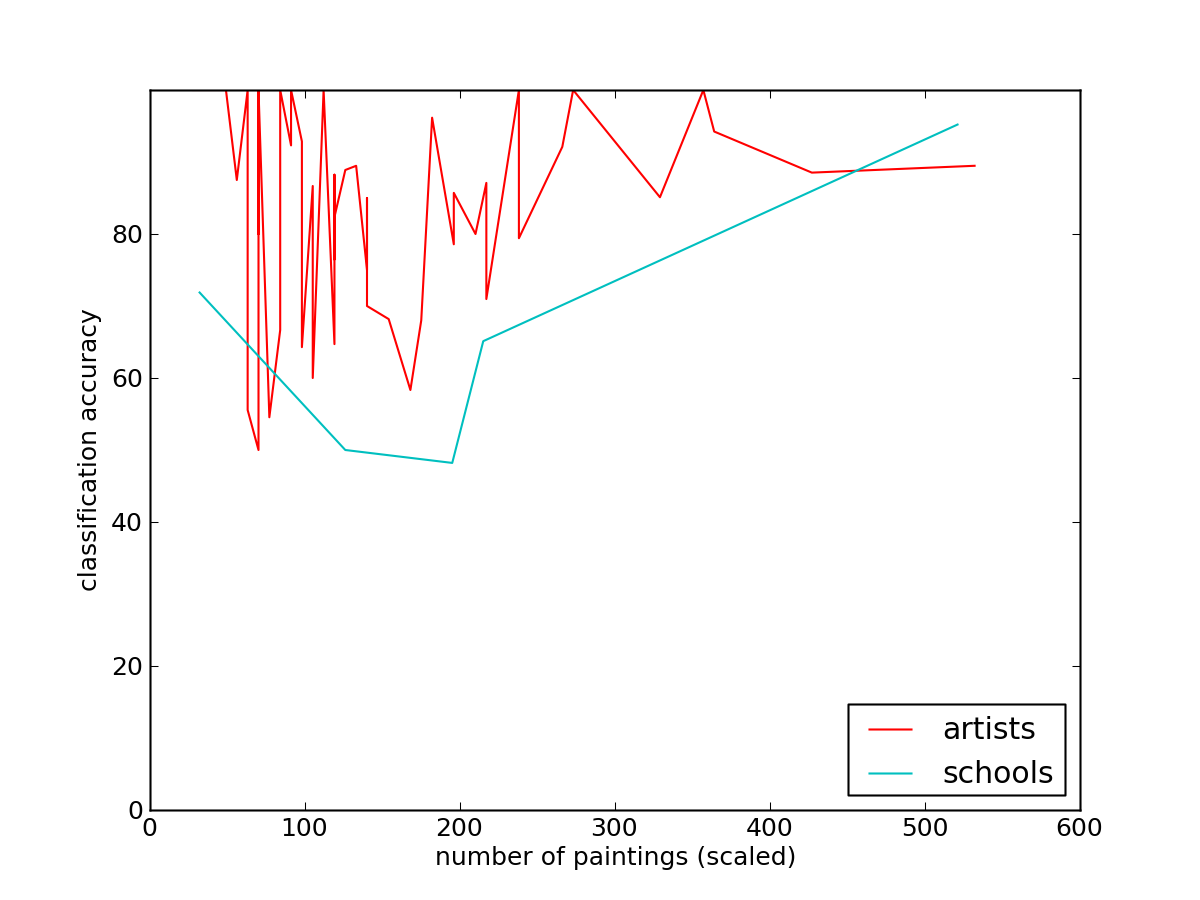
\includegraphics[width=0.7\textwidth]{class-graph}
\caption[Classification]{Classification Accuracy}
\label{fig:class}
\end{figure*}

\begin{figure*}[tbp]
\centering
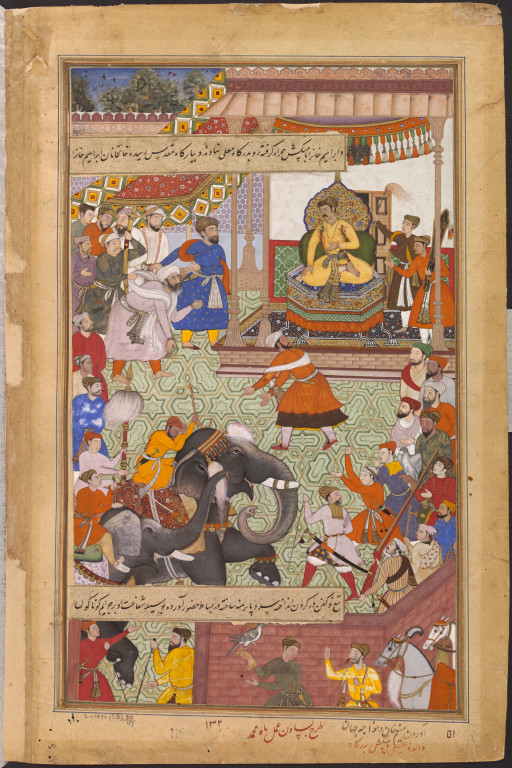
\includegraphics[width=0.30\textwidth]{basawan_2009BX3686}
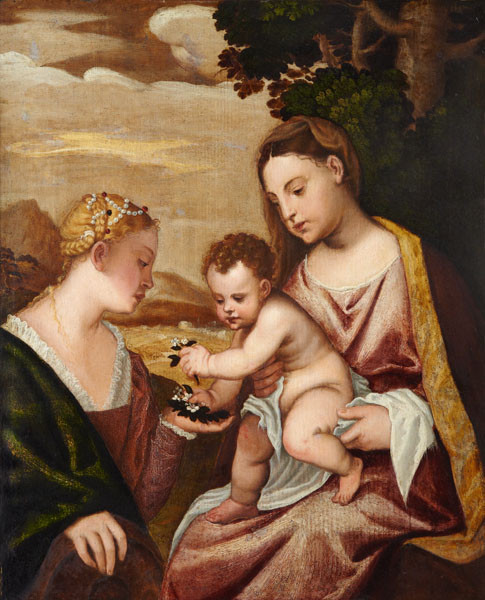
\includegraphics[width=0.30\textwidth]{titian_eu_741}
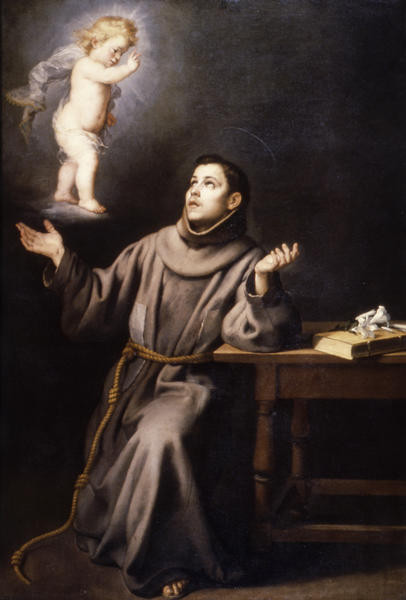
\includegraphics[width=0.30\textwidth]{murillo_1974p24}
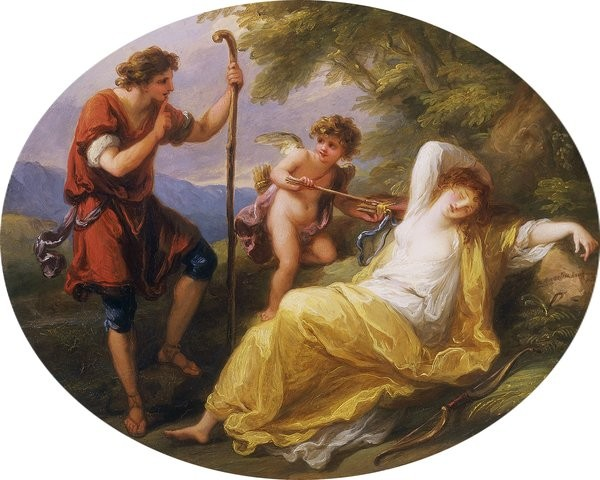
\includegraphics[width=0.48\textwidth]{kauffmann_va_pc_2006an1773}
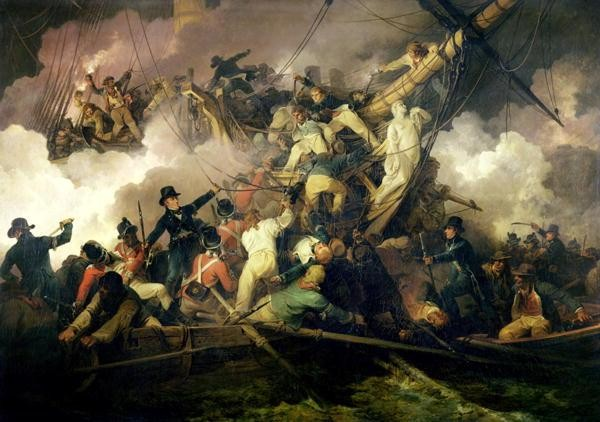
\includegraphics[width=0.48\textwidth]{loutherbourg_k264}
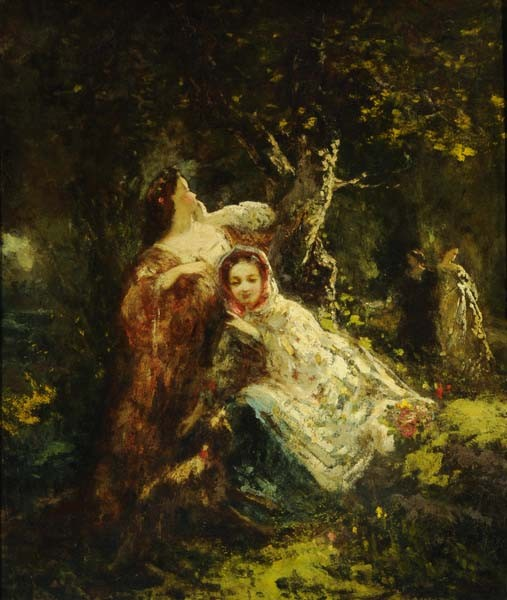
\includegraphics[width=0.40\textwidth]{monticelli_300}
\caption[Examples of styles in art movements/schools]{Styles}
\label{fig:styles}
\end{figure*}

\chapter{Conclusions}

Whelp, it will be some time before I write this.

\end{multicols}

\newpage
\phantomsection
\addcontentsline{toc}{chapter}{\bibname}
\bibliographystyle{plain}
\bibliography{capybara}

\appendix

\chapter{Requirements to run the code}
\label{chap:requirements}

Describe each library installed, there are some.

Compiled software (often available as software packages as .rpm or .deb)
\begin{itemize}
\item[]\emph{ImageMagick} 6.5.4-7 or later, \\
available at \href{http://www.imagemagick.org/}{http://www.imagemagick.org/}

\item[]\emph{libsvm} 3.18 or later, \\
available at \href{http://csie.ntu.edu.tw/~cjlin/libsvm/index}
{http://csie.ntu.edu.tw/~cjlin/libsvm/index}
\end{itemize}

Provided by LSB:
\begin{itemize}
\item[]\emph{python} 2.6.6 or later (but not python 3), \\
available at \href{http://www.python.org/}{http://www.python.org/}

\item[]\emph{perl} 5.8.8 or later, \\
available at \href{http://www.perl.org/}{http://www.perl.org/}

\item[]\emph{bash} 4.1.0 or later, \\
available at \href{http://www.gnu.org/software/bash/index.html}
{http://www.gnu.org/software/bash/index.html}
\end{itemize}

Python packages:
\begin{itemize}
\item[]\emph{numpy} 1.8.1 or later, \\
available at \href{http://www.numpy.org/}{http://www.numpy.org/}

\item[]\emph{scipy} 0.14.0, \\
available at \href{http://www.scipy.org/}{http://www.scipy.org/}

\item[]\emph{matplotlib} 0.99.1.1, \\
available at \href{http://matplotlib.org/}{http://matplotlib.org/}

\item[]\emph{pillow} 2.5.1 or later, \\
available at the pypi index at
\href{https://pypi.python.org/pypi/Pillow}
{http://pypi.python.org/pypi/Pillow} \\
or directly from github at
\href{http://github.com/python-pillow/Pillow}
{http://github.com/python-pillow/Pillow}

\item[]\emph{scikit-image} 0.10.1, \\
available at \href{http://scikit-image.org/}{http://scikit-image.org/}

\item[]\emph{ipython} 1.0.0 or later, \\
available at \href{http://ipython.org/}{http://ipython.org/}

\item[]\emph{pandas} 0.14.1, \\
available at \href{http://pandas.pydata.org/}{http://pandas.pydata.org/}
\end{itemize}

For dataset acquisition
\begin{itemize}
\item[]\emph{beautifulsoup4} 4.3.2 or later, \\
available at \href{http://www.crummy.com/software/BeautifulSoup/}
{http://www.crummy.com/software/BeautifulSoup/}

\item[]\emph{pyyaml} 3.10 or later, \\
available at \href{http://pyyaml.org/}{http://pyyaml.org/}

\item[]\emph{git} 1.5.0 or later is needed to clone unixjsons from its
repository, available at \href{http://www.git-scm.com/}{http://www.git-scm.com/}

\item[]\emph{unixjsons} 0.7 or later, \\
available at \href{https://github.com/grochmal/unixjsons}
{https://github.com/grochmal/unixjsons}
\end{itemize}

\chapter{How to run the code}
\label{chap:runthecode}

Before running the code make sure you are in an LSB compatible system\footnote{
\href{http://www.linuxfoundation.org/collaborate/workgroups/lsb}
{http://www.linuxfoundation.org/collaborate/workgroups/lsb}} and install the
libraries described in Appendix \ref{chap:requirements}.  Copy the code into a
directory\footnote{If git and an internet connection are available you can
clone the code directly from its repository with
\verb|git clone https://github.com/grochmal/capybara.git|.}
and go to \texttt{src/}.

Acquisition and cleansing of the datasets is not covered because that process
is not automated.  To browse the code used to acquire the datasets go to
\texttt{dataset-acquisition/vam} and \texttt{dataset-acquisition/nirp} for the
VAM and NIRP datasets respectively.

In \texttt{src/} run the scripts that normalise, separate and filter the images
before the extraction of features:

\begin{Verbatim}[frame=leftline]
./step01-normalise.sh      # normalise to ~300 000 pixels
./step02-hsl-hsv.sh        # separates the channels
./step03-colourfulness.sh  # calculates the colourfulness
./step04-sobel.sh          # applies the Sobel filter
./step05-canny.sh          # applies the Canny filter
./step06-jpeg.sh           # compress the images
\end{Verbatim}

Next run the feature extractors.  These scripts print the calculated features
to the \emph{standard output stream} and logging to the \emph{standard error
stream}, therefore redirect the standard output to files:

\begin{Verbatim}[frame=leftline]
./step07-kolmogorov.sh     > fe/kolmogorov.dat
./step08-glcm.sh           > fe/glcm.dat
./step09-itten12.sh        > fe/itten12.dat
./step10-itten-contrast.sh > fe/itten-contrast.dat
./step11-rule-of-3.sh      > fe/rule-of-3.dat
./step12-img-averages.sh   > fe/img-averages.dat
\end{Verbatim}

A last feature script generating the metadata (artist, school and contry) of
the image shall then be run.  This metadata is what we classify against:

\begin{Verbatim}[frame=leftline]
./step13-metadata.sh > fe/meta.dat
\end{Verbatim}

Format the features to a format compatible with LIBSVM and run the classifiers
using the following scripts.  The results of the classifiers are printed to the
file \texttt{cls/output.dat}.

\begin{Verbatim}[frame=leftline]
./step14-libsvm-format.sh
./step15-classify.sh
\end{Verbatim}

The last script combines the results from the classifiers and the full dataset
of features (the horizontal concatenation of all \texttt{.dat} files) to
produce the graphs and tables present in Chapter \ref{chap:results} and
Appendix \ref{chap:glossary}.

\begin{Verbatim}[frame=leftline]
./step16-outputs.sh
\end{Verbatim}

\chapter{unixjsons}
\label{chap:unixjsons}

\section{jgrep}

Amount of noise (by random sample) in the cleansed datasets.

Start writing about dataset cleansing heuristics, plus some *descriptions* and
*statistics*.

Get some of the artists (with most paintings) and do some statistics over
those.

Histograms of features (especially itten colours) by different artists.

R library to explore data: ggplot2 (use it?).

% Inside \small Verbatim use 69 characters max to respect the margins
{\small
\begin{Verbatim}[samepage=true]
Usage: jgrep [-n key] [-hVqviIHR] <key re> <value re> [<file> ...]

  -h, --help
        Print this help.

  -V, --version
        Prints the version of the script.

  -q, --quiet, --silent
        Do not print anything, even on error.

  -n key, --line-number=key
        Give the line number in the output, it is added to the
        result under the key specified as the argument.

  -v, --invert-match
        Print lines that do not match re pattern pattern.
\end{Verbatim}
}

\section{jcut}

nanan nanan nanan nanan nanan nanan nanan nanan nanan nanan nanan nanan nanan
nanan nanan nanan nanan nanan nanan nanan nanan nanan nanan nanan nanan nanan
nanan nanan nanan nanan nanan nanan nanan nanan nanan nanan nanan nanan nanan
nanan nanan nanan nanan nanan nanan nanan nanan nanan nanan nanan nanan nanan
nanan nanan nanan nanan nanan nanan nanan nanan nanan nanan nanan nanan nanan
nanan nanan nanan nanan nanan nanan nanan nanan nanan nanan nanan nanan nanan
nanan nanan nanan nanan nanan nanan nanan nanan nanan nanan nanan nanan nanan
nanan nanan nanan nanan nanan nanan nanan nanan nanan nanan nanan nanan nanan
nanan nanan nanan nanan nanan nanan nanan nanan nanan nanan nanan nanan nanan
batman

{\small
\begin{Verbatim}[samepage=true]
Usage: jcut [-chrlV] [-f field,field,...] [<file> ...]

  -h, --help
        Print this help.

  -V, --version
        Prints the version of the script.

  -f, --fields=
        Comma delimited list of fields to cut from the JSON.

  -c, --complement
        Print all fields that are not in the fields list.

  -r, --regex
        Treat every field in the field list as a regex, this
        is useful to pattern match several similar fields or
        to match a field with a comma in it (using \\054).

  -l, --list
        Print all available field in the input, then exit.
\end{Verbatim}
}

\section{jsed}

A simplified implementation of \texttt{sed} command that works on a JSONS
stream.  It implements the \texttt{s///} substitution command for several
combinations of key and value pair combinations.  Both keys and values can be
matched and/or changed using substitution regular expressions.  The usage of
\texttt{jsed}, including some examples follows:

{\small
\begin{verbatim}
Usage: jsed [-hVqiI] [-f file | -e expr -e expr ...] [<file> ...]

  -h, --help
        Print this help.

  -V, --version
        Prints the version of the script.

  -q, --quiet, --silent
        Do not print anything, even on error.

  -e /pattern/replacement/, --expression=/pattern/replacement/
  -e /pattern/replacement/flags
  -e /pattern/pattern/replacement/
  -e /pattern/pattern/replacement/flags
  -e /pattern/replacement/pattern/replacement/
  -e /pattern/replacement/pattern/replacement/flags
  -e {pattern}{replacement}
  -e {pattern}{replacement}flags
  -e {pattern}{pattern}{replacement}
  -e {pattern}{pattern}{replacement}flags
  -e {pattern}{replacement}{pattern}{replacement}
  -e {pattern}{replacement}{pattern}{replacement}flags
        The substitution expression to execute, this expression
        will be run on every line on every key that matches.
        Several expressions can be specified on a single
        invocation and will be executed in the order they're
        present in the command line.  The pattern part of the
        expression is a regular expression, whilst the
        replacement part is a string that accepts '\'
        groupings (e.g. \1 for first grouping).

        An expression is divided into fields, each field is
        delimited by a delimiter character.  The first character
        of the expression becomes the delimiter character, every
        occurrence of that character thereof will mark the start
        of a new field.  The delimiter character must be
        printable and cannot be a digit (0-9) or one of the
        characters: 'g', 'i', '.' or '#'.  The delimiter
        character cannot be used in the fields of the
        expression.

        Also, the three grouping pairs characters '()', '[]'
        and '{}' can be used to group the fields together.
        Note that using '()' will not allow the use of grouping
        in the pattern and using '[]' will not allow the use of
        character definitions.

        Examples of equivalent expressions follows:

        Change the key 'image_id' to 'image':
            -e /image_id/image/
            -e ;image_id;image;
            -e "image_id"image"
            -e {image_id}{image}
            -e (image_id)(image)

        Every image key content from .jpg to .png
            -e /image_.*/\.jpg$/.png/g
            -e =image_.*=\.jpg$=.png=g
            -e [image_.*][\.jpg$][.png]g

        First change every field containing `image` to start
        with this word, then change every occurrence of .jpg
        to .png (note: if two fields are named `first_image`,
        `second_image` the first field will be overridden by
        the second because the substitution happens in
        ASCIIbetical order of fields).
            -e /.*image(.*)/image\1/g -e /image.*/\.jpg/.png/g
            -e {.*image(.*)}{image\1}g -e {image.*}{\.jpg}{.png}g
            -e /.*image(.*)/image\1/g -e {image.*}{\.jpg}{.png}g

        More on the purpose of each field  and the `flags`
        suffix in the -e expression can be found in the
        `Expression` section, below.

  -f script_file, --file=script_file
        The script file contains one expression (as in the -e
        option) per line, which are executed in order as they
        appear in the input.  Every expression in the
        `script_file` is exactly the same as if it was passed
        to the -e flag.

        If both -f and -e are present (possibly several -e
        flags) the changes to each line of the input will
        happen by first executing the script passed by -f
        and then executing all -e flags in order.

  -i, --in-place
        Change the file in place, the default is to print the
        modified file to standard output.  If the input is
        composed of standard input only, of several files or
        of a combination of standard input and files this flag
        is ignored.

  -b extension , --backup=extension
        If -i is in effect copy the input file is copied and the
        extension `extension` is appended to it.  Only then the
        original file is modified.  If -i is in effect and -b is
        not present the changes made are irreversible.
\end{verbatim}
}

\section{jecho}

nanan nanan nanan nanan nanan nanan nanan nanan nanan nanan nanan nanan nanan
nanan nanan nanan nanan nanan nanan nanan nanan nanan nanan nanan nanan nanan
nanan nanan nanan nanan nanan nanan nanan nanan nanan nanan nanan nanan nanan
nanan nanan nanan nanan nanan nanan nanan nanan nanan nanan nanan nanan nanan
nanan nanan nanan nanan nanan nanan nanan nanan nanan nanan nanan nanan nanan
nanan nanan nanan nanan nanan nanan nanan nanan nanan nanan nanan nanan nanan
nanan nanan nanan nanan nanan nanan nanan nanan nanan nanan nanan nanan nanan
nanan nanan nanan nanan nanan nanan nanan nanan nanan nanan nanan nanan nanan
nanan nanan nanan nanan nanan nanan nanan nanan nanan nanan nanan nanan nanan
batman

{\small
\begin{Verbatim}[samepage=true]
Usage: jecho [-hV] -f k:v [-f k:v -f k:v ...] [<file> ...]

  -h, --help
        Print this help.

  -V, --version
        Prints the version of the script.

  -q, --quiet, --silent
        Do not print messages.

  -f k:v, --field=k:v
        Add field `k` with value `v` to the stream.

  -r, --replace
        By default fields already in the stream will not be
        replaced, unless this flag is on.
\end{Verbatim}
}

\section{jjoin}

nanan nanan nanan nanan nanan nanan nanan nanan nanan nanan nanan nanan nanan
nanan nanan nanan nanan nanan nanan nanan nanan nanan nanan nanan nanan nanan
nanan nanan nanan nanan nanan nanan nanan nanan nanan nanan nanan nanan nanan
nanan nanan nanan nanan nanan nanan nanan nanan nanan nanan nanan nanan nanan
nanan nanan nanan nanan nanan nanan nanan nanan nanan nanan nanan nanan nanan
nanan nanan nanan nanan nanan nanan nanan nanan nanan nanan nanan nanan nanan
nanan nanan nanan nanan nanan nanan nanan nanan nanan nanan nanan nanan nanan
nanan nanan nanan nanan nanan nanan nanan nanan nanan nanan nanan nanan nanan
nanan nanan nanan nanan nanan nanan nanan nanan nanan nanan nanan nanan nanan
batman

{\small
\begin{Verbatim}[samepage=true]
Usage: jjoin [-hVq] file1 file2

  -h, --help
        Print this help.

  -V, --version
        Prints the version of the script.

  -q, --quiet, --silent
        Do not print messages.

  -, STDIN
        Read from STDIN instead of file.
\end{Verbatim}
}

\chapter{Resources on the CD}
\label{chap:resources}

The DVD contains the cleaned datasets and the code to run all experiments under
a directory called \texttt{capybara}.  That directory also contains a README.md
file which mentions the Copyright (Copyleft) of the code and explains how to
run it, in the same way as Appendix \ref{chap:runthecode}.  The CD also
contains a copy of the code of \emph{unixjsons}, which is needed to browse the
intermediate files in acquiring the datasets.  \emph{unixjsons} is mentioned in
Appendix \ref{chap:unixjsons}.

If the CD is not available the code for the experiments can be retrieved using
\emph{git}:

\begin{verbatim}
git clone https://github.com/grochmal/capybara.git
\end{verbatim}

Also, a mentioned in Appendix \ref{chap:unixjsons}, the code for
\emph{unixjsons} can be retrieved using \emph{git} too:

\begin{verbatim}
git clone https://github.com/grochmal/unixjsons.git
\end{verbatim}

\newpage
\null
\thispagestyle{empty}
\newpage

\chapter{Feature Values}
\label{chap:glossary}

Table \ref{tab:glossary} present a glossary of all features used, this shall be
used as a reference for reading the legends and graphs.  Tables
\ref{tab:bigtop} and \ref{tab:bigbot} show mean values of each feature
aggregated by the art school.

\begin{center}
\footnotesize
\begin{longtable}{|l|c|l|}
\toprule
\multirow{2}{*}{Feature} & number   & short name         \\
                         & (graphs) & (in the data file) \\
\midrule
\endhead

\midrule
\multicolumn{3}{r}{{Continued on next page}} \\
\cmidrule{2-3}
\endfoot

\bottomrule
\caption[Feature glossary]{Glossary of all features, divided into the feature
groups described.  For each feature the short name used in legends and tables
is shown, as well as the id (number) of the feature used in graphs.}
\label{tab:glossary}
\endlastfoot

\midrule
\multicolumn{3}{c}{Komogorov Complexity for$\ldots$} \\
\midrule
Colourfulness (quality 60)                      &  0 & nofilter-cs60   \\
Colourfulness (quality 40)                      &  1 & nofilter-cs40   \\
Colourfulness (quality 20)                      &  2 & nofilter-cs20   \\
Hue (quality 60)                                &  3 & nofilter-h60    \\
Hue (quality 40)                                &  4 & nofilter-h40    \\
Hue (quality 20)                                &  5 & nofilter-h20    \\
Lightness (quality 60)                          &  6 & nofilter-l60    \\
Lightness (quality 40)                          &  7 & nofilter-l40    \\
Lightness (quality 20)                          &  8 & nofilter-l20    \\
Saturation$_{HSV}$ (quality 60)                 &  9 & nofilter-shsv60 \\
Saturation$_{HSV}$ (quality 40)                 & 10 & nofilter-shsv40 \\
Saturation$_{HSV}$ (quality 20)                 & 11 & nofilter-shsv20 \\
Saturation$_{HSL}$ (quality 60)                 & 12 & nofilter-shsl60 \\
Saturation$_{HSL}$ (quality 40)                 & 13 & nofilter-shsl40 \\
Saturation$_{HSL}$ (quality 20)                 & 14 & nofilter-shsl20 \\
Value (quality 60)                              & 15 & nofilter-v60    \\
Value (quality 40)                              & 16 & nofilter-v40    \\
Value (quality 20)                              & 17 & nofilter-v20    \\
Sobel filter of Colourfulness (quality 60)      & 18 & sobel-cs60      \\
Sobel filter of Colourfulness (quality 40)      & 19 & sobel-cs40      \\
Sobel filter of Colourfulness (quality 20)      & 20 & sobel-cs20      \\
Sobel filter of Hue (quality 60)                & 21 & sobel-h60       \\
Sobel filter of Hue (quality 40)                & 22 & sobel-h40       \\
Sobel filter of Hue (quality 20)                & 23 & sobel-h20       \\
Sobel filter of Lightness (quality 60)          & 24 & sobel-l60       \\
Sobel filter of Lightness (quality 40)          & 25 & sobel-l40       \\
Sobel filter of Lightness (quality 20)          & 26 & sobel-l20       \\
Sobel filter of Saturation$_{HSV}$ (quality 60) & 27 & sobel-shsv60    \\
Sobel filter of Saturation$_{HSV}$ (quality 40) & 28 & sobel-shsv40    \\
Sobel filter of Saturation$_{HSV}$ (quality 20) & 29 & sobel-shsv20    \\
Sobel filter of Saturation$_{HSL}$ (quality 60) & 30 & sobel-shsl60    \\
Sobel filter of Saturation$_{HSL}$ (quality 40) & 31 & sobel-shsl40    \\
Sobel filter of Saturation$_{HSL}$ (quality 20) & 32 & sobel-shsl20    \\
Sobel filter of Value (quality 60)              & 33 & sobel-v60       \\
Sobel filter of Value (quality 40)              & 34 & sobel-v40       \\
Sobel filter of Value (quality 20)              & 35 & sobel-v20       \\
Canny filter of Colourfulness (quality 60)      & 36 & canny-cs60      \\
Canny filter of Colourfulness (quality 40)      & 37 & canny-cs40      \\
Canny filter of Colourfulness (quality 20)      & 38 & canny-cs20      \\
Canny filter of Hue (quality 60)                & 39 & canny-h60       \\
Canny filter of Hue (quality 40)                & 40 & canny-h40       \\
Canny filter of Hue (quality 20)                & 41 & canny-h20       \\
Canny filter of Lightness (quality 60)          & 42 & canny-l60       \\
Canny filter of Lightness (quality 40)          & 43 & canny-l40       \\
Canny filter of Lightness (quality 20)          & 44 & canny-l20       \\
Canny filter of Saturation$_{HSV}$ (quality 60) & 45 & canny-shsv60    \\
Canny filter of Saturation$_{HSV}$ (quality 40) & 46 & canny-shsv40    \\
Canny filter of Saturation$_{HSV}$ (quality 20) & 47 & canny-shsv20    \\
Canny filter of Saturation$_{HSL}$ (quality 60) & 48 & canny-shsl60    \\
Canny filter of Saturation$_{HSL}$ (quality 40) & 49 & canny-shsl40    \\
Canny filter of Saturation$_{HSL}$ (quality 20) & 50 & canny-shsl20    \\
Canny filter of Value (quality 60)              & 51 & canny-v60       \\
Canny filter of Value (quality 40)              & 52 & canny-v40       \\
Canny filter of Value (quality 20)              & 53 & canny-v20       \\

\midrule
\multicolumn{3}{c}{Grey Level Co-occurence Matrix} \\
\midrule
Contrast of Colourfulness (each pixel)             &  54 & glcm-cs-ct1    \\
Contrast of Colourfulness (each 6 pixels)          &  55 & glcm-cs-ct6    \\
Contrast of Colourfulness (each 20 pixels)         &  56 & glcm-cs-ct20   \\
Energy of Colourfulness (each pixel)               &  57 & glcm-cs-en1    \\
Energy of Colourfulness (each 6 pixels)            &  58 & glcm-cs-en6    \\
Energy of Colourfulness (each 20 pixels)           &  59 & glcm-cs-en20   \\
Homogeneity of Colourfulness (each pixel)          &  60 & glcm-cs-hm1    \\
Homogeneity of Colourfulness (each 6 pixels)       &  61 & glcm-cs-hm6    \\
Homogeneity of Colourfulness (each 20 pixels)      &  62 & glcm-cs-hm20   \\
Correlation of Colourfulness (each pixel)          &  63 & glcm-cs-cr1    \\
Correlation of Colourfulness (each 6 pixels)       &  64 & glcm-cs-cr6    \\
Correlation of Colourfulness (each 20 pixels)      &  65 & glcm-cs-cr20   \\
Contrast of Hue (each pixel)                       &  66 & glcm-h-ct1     \\
Contrast of Hue (each 6 pixels)                    &  67 & glcm-h-ct6     \\
Contrast of Hue (each 20 pixels)                   &  68 & glcm-h-ct20    \\
Energy of Hue (each pixel)                         &  69 & glcm-h-en1     \\
Energy of Hue (each 6 pixels)                      &  70 & glcm-h-en6     \\
Energy of Hue (each 20 pixels)                     &  71 & glcm-h-en20    \\
Homogeneity of Hue (each pixel)                    &  72 & glcm-h-hm1     \\
Homogeneity of Hue (each 6 pixels)                 &  73 & glcm-h-hm6     \\
Homogeneity of Hue (each 20 pixels)                &  74 & glcm-h-hm20    \\
Correlation of Hue (each pixel)                    &  75 & glcm-h-cr1     \\
Correlation of Hue (each 6 pixels)                 &  76 & glcm-h-cr6     \\
Correlation of Hue (each 20 pixels)                &  77 & glcm-h-cr20    \\
Contrast of Lightness (each pixel)                 &  78 & glcm-l-ct1     \\
Contrast of Lightness (each 6 pixels)              &  79 & glcm-l-ct6     \\
Contrast of Lightness (each 20 pixels)             &  80 & glcm-l-ct20    \\
Energy of Lightness (each pixel)                   &  81 & glcm-l-en1     \\
Energy of Lightness (each 6 pixels)                &  82 & glcm-l-en6     \\
Energy of Lightness (each 20 pixels)               &  83 & glcm-l-en20    \\
Homogeneity of Lightness (each pixel)              &  84 & glcm-l-hm1     \\
Homogeneity of Lightness (each 6 pixels)           &  85 & glcm-l-hm6     \\
Homogeneity of Lightness (each 20 pixels)          &  86 & glcm-l-hm20    \\
Correlation of Lightness (each pixel)              &  87 & glcm-l-cr1     \\
Correlation of Lightness (each 6 pixels)           &  88 & glcm-l-cr6     \\
Correlation of Lightness (each 20 pixels)          &  89 & glcm-l-cr20    \\
Contrast of Saturation$_{HSL}$ (each pixel)        &  90 & glcm-shsl-ct1  \\
Contrast of Saturation$_{HSL}$ (each 6 pixels)     &  91 & glcm-shsl-ct6  \\
Contrast of Saturation$_{HSL}$ (each 20 pixels)    &  92 & glcm-shsl-ct20 \\
Energy of Saturation$_{HSL}$ (each pixel)          &  93 & glcm-shsl-en1  \\
Energy of Saturation$_{HSL}$ (each 6 pixels)       &  94 & glcm-shsl-en6  \\
Energy of Saturation$_{HSL}$ (each 20 pixels)      &  95 & glcm-shsl-en20 \\
Homogeneity of Saturation$_{HSL}$ (each pixel)     &  96 & glcm-shsl-hm1  \\
Homogeneity of Saturation$_{HSL}$ (each 6 pixels)  &  97 & glcm-shsl-hm6  \\
Homogeneity of Saturation$_{HSL}$ (each 20 pixels) &  98 & glcm-shsl-hm20 \\
Correlation of Saturation$_{HSL}$ (each pixel)     &  99 & glcm-shsl-cr1  \\
Correlation of Saturation$_{HSL}$ (each 6 pixels)  & 100 & glcm-shsl-cr6  \\
Correlation of Saturation$_{HSL}$ (each 20 pixels) & 101 & glcm-shsl-cr20 \\
Contrast of Saturation$_{HSV}$ (each pixel)        & 102 & glcm-shsv-ct1  \\
Contrast of Saturation$_{HSV}$ (each 6 pixels)     & 103 & glcm-shsv-ct6  \\
Contrast of Saturation$_{HSV}$ (each 20 pixels)    & 104 & glcm-shsv-ct20 \\
Energy of Saturation$_{HSV}$ (each pixel)          & 105 & glcm-shsv-en1  \\
Energy of Saturation$_{HSV}$ (each 6 pixels)       & 106 & glcm-shsv-en6  \\
Energy of Saturation$_{HSV}$ (each 20 pixels)      & 107 & glcm-shsv-en20 \\
Homogeneity of Saturation$_{HSV}$ (each pixel)     & 108 & glcm-shsv-hm1  \\
Homogeneity of Saturation$_{HSV}$ (each 6 pixels)  & 109 & glcm-shsv-hm6  \\
Homogeneity of Saturation$_{HSV}$ (each 20 pixels) & 110 & glcm-shsv-hm20 \\
Correlation of Saturation$_{HSV}$ (each pixel)     & 111 & glcm-shsv-cr1  \\
Correlation of Saturation$_{HSV}$ (each 6 pixels)  & 112 & glcm-shsv-cr6  \\
Correlation of Saturation$_{HSV}$ (each 20 pixels) & 113 & glcm-shsv-cr20 \\
Contrast of Value (each pixel)                     & 114 & glcm-v-ct1     \\
Contrast of Value (each 6 pixels)                  & 115 & glcm-v-ct6     \\
Contrast of Value (each 20 pixels)                 & 116 & glcm-v-ct20    \\
Energy of Value (each pixel)                       & 117 & glcm-v-en1     \\
Energy of Value (each 6 pixels)                    & 118 & glcm-v-en6     \\
Energy of Value (each 20 pixels)                   & 119 & glcm-v-en20    \\
Homogeneity of Value (each pixel)                  & 120 & glcm-v-hm1     \\
Homogeneity of Value (each 6 pixels)               & 121 & glcm-v-hm6     \\
Homogeneity of Value (each 20 pixels)              & 122 & glcm-v-hm20    \\
Correlation of Value (each pixel)                  & 123 & glcm-v-cr1     \\
Correlation of Value (each 6 pixels)               & 124 & glcm-v-cr6     \\
Correlation of Value (each 20 pixels)              & 125 & glcm-v-cr20    \\

\midrule
\multicolumn{3}{c}{Itten Colours} \\
\midrule
Amount of Red           & 126 & it12-r  \\
Amount of Orange Red    & 127 & it12-or \\
Amount of Orange        & 128 & it12-o  \\
Amount of Orange Yellow & 129 & it12-oy \\
Amount of Yellow        & 130 & it12-y  \\
Amount of Green Yellow  & 131 & it12-gy \\
Amount of Green         & 132 & it12-g  \\
Amount of Green Blue    & 133 & it12-gb \\
Amount of Blue          & 134 & it12-b  \\
Amount of Purple Blue   & 135 & it12-pb \\
Amount of Purple        & 136 & it12-p  \\
Amount of Purple Red    & 137 & it12-pr \\

\midrule
\multicolumn{3}{c}{Rule of Thirds} \\
\midrule
Average of central Colourfulness                 & 138 & r3-cs-avg   \\
Standard Deviation of central Colourfulness      & 139 & r3-cs-std   \\
Average of central Hue                           & 140 & r3-h-avg    \\
Standard Deviation of central Hue                & 141 & r3-h-std    \\
Average of central Lightness                     & 142 & r3-l-avg    \\
Standard Deviation of central Lightness          & 143 & r3-l-std    \\
Average of central Saturation$_{HSL}$            & 144 & r3-shsl-avg \\
Standard Deviation of central Saturation$_{HSL}$ & 145 & r3-shsl-std \\
Average of central Saturation$_{HSV}$            & 146 & r3-shsv-avg \\
Standard Deviation of central Saturation$_{HSV}$ & 147 & r3-shsv-std \\
Average of central Value                         & 148 & r3-v-avg    \\
Standard Deviation of central Value              & 149 & r3-v-std    \\

\midrule
\multicolumn{3}{c}{Itten Contrast of$\ldots$} \\
\midrule
Saturation$_{HSL}$ (rule of thirds)              & 150 & itct-sat-sl-r3      \\
Saturation$_{HSL}$ (rule of sevenths)            & 151 & itct-sat-sl-r7      \\
Saturation$_{HSL}$ (watershed)                   & 152 & itct-sat-sl-sg      \\
Saturation$_{HSV}$ (rule of thirds)              & 153 & itct-sat-sv-r3      \\
Saturation$_{HSV}$ (rule of sevenths)            & 154 & itct-sat-sv-r7      \\
Saturation$_{HSV}$ (watershed)                   & 155 & itct-sat-sv-sg      \\
Light and Dark of Lightness (rule of thirds)     & 156 & itct-lightdark-l-r3 \\
Light and Dark of Lightness (rule of sevenths)   & 157 & itct-lightdark-l-r7 \\
Light and Dark of Lightness (watershed)          & 158 & itct-lightdark-l-sg \\
Light and Dark of Value (rule of thirds)         & 159 & itct-lightdark-v-r3 \\
Light and Dark of Value (rule of sevenths)       & 160 & itct-lightdark-v-r7 \\
Light and Dark of Value (watershed)              & 161 & itct-lightdark-v-sg \\
Hue (rule of thirds)                             & 162 & itct-hue-h-r3       \\
Hue (rule of sevenths)                           & 163 & itct-hue-h-r7       \\
Hue (watershed)                                  & 164 & itct-hue-h-sg       \\
Hue Colourfulness (rule of thirds)               & 165 & itct-hue-cs-r3      \\
Hue Colourfulness (rule of sevenths)             & 166 & itct-hue-cs-r7      \\
Hue Colourfulness (watershed)                    & 167 & itct-hue-cs-sg      \\
Warm and Cold of Hue (rule of thirds)            & 168 & itct-warmcold-h-r3  \\
Warm and Cold of Hue (rule of sevenths)          & 169 & itct-warmcold-h-r7  \\
Warm and Cold of Hue (watershed)                 & 170 & itct-warmcold-h-sg  \\
Warm and Cold of Colourfulness (rule of thirds)  & 171 & itct-warmcold-cs-r3 \\
Warm and Cold of Colourfulness (rule of sevenths)& 172 & itct-warmcold-cs-r7 \\
Warm and Cold of Colourfulness (watershed)       & 173 & itct-warmcold-cs-sg \\
Complements of Hue (rule of thirds)              & 174 & itct-comp-h-r3      \\
Complements of Hue (rule of sevenths)            & 175 & itct-comp-h-r7      \\
Complements of Hue (watershed)                   & 176 & itct-comp-h-sg      \\
Complements of Colourfulness (rule of thirds)    & 177 & itct-comp-cs-r3     \\
Complements of Colourfulness (rule of sevenths)  & 178 & itct-comp-cs-r7     \\
Complements of Colourfulness (watershed)         & 179 & itct-comp-cs-sg     \\

\midrule
\multicolumn{3}{c}{Image Averages} \\
\midrule
Average of Colourfulness                 & 180 & cs-avg   \\
Standard Deviation of Colourfulness      & 181 & cs-std   \\
Average of Hue                           & 182 & h-avg    \\
Standard Deviation of Hue                & 183 & h-std    \\
Average of Lightness                     & 184 & l-avg    \\
Standard Deviation of Lightness          & 185 & l-std    \\
Average of Saturation$_{HSL}$            & 186 & shsl-avg \\
Standard Deviation of Saturation$_{HSL}$ & 187 & shsl-std \\
Average of Saturation$_{HSV}$            & 188 & shsv-avg \\
Standard Deviation of Saturation$_{HSV}$ & 189 & shsv-std \\
Average of Value                         & 190 & v-avg    \\
Standard Deviation of Value              & 191 & v-std    \\
\bottomrule
\end{longtable}
\end{center}

\newpage

\begin{center}
\footnotesize
\begin{longtable}{l|rr|rr|rr}
\toprule
\multirow{2}{*}{Feature}
  & \multicolumn{2}{c}{renaissance}
  & \multicolumn{2}{c}{baroque}
  & \multicolumn{2}{c}{neoclassicism}
  \\
\cline{2-7}
& mean & std & mean & std & mean & std \\
\midrule
\endhead

\midrule
\multicolumn{3}{r}{} \\
\multicolumn{3}{r}{{Continued on next page}} \\
\multicolumn{3}{r}{} \\
\midrule
\endfoot

\bottomrule
\caption[Feature values (first half)]{Mean and standard deviation of all
features grouped by the art schools of renaissance, baroque and neoclassicism.
The features are identified by the short names from table \ref{tab:glossary}.}
\label{tab:bigtop}
\endlastfoot

\begin{tabular}{lrrrrrr}
\toprule
kol-nofilter-cs60   &   14.45 &    4.36 &   16.60 &    5.77 &   15.46 &    5.62 \\
\midrule
kol-nofilter-cs40   &   19.62 &    6.12 &   22.92 &    8.28 &   21.43 &    8.05 \\
kol-nofilter-cs20   &   32.55 &   10.74 &   39.00 &   14.81 &   36.94 &   14.70 \\
kol-nofilter-h60    &   13.37 &    7.19 &   15.45 &    8.50 &   17.44 &    8.38 \\
kol-nofilter-h40    &   18.78 &   11.28 &   22.19 &   13.45 &   25.41 &   13.50 \\
kol-nofilter-h20    &   33.20 &   23.02 &   40.58 &   27.69 &   47.38 &   28.54 \\
kol-nofilter-l60    &    9.16 &    2.54 &   10.18 &    2.83 &    9.32 &    2.87 \\
kol-nofilter-l40    &   12.36 &    3.78 &   13.94 &    4.11 &   12.69 &    4.03 \\
kol-nofilter-l20    &   20.80 &    7.25 &   24.08 &    7.51 &   21.78 &    7.05 \\
kol-nofilter-shsv60 &    6.11 &    5.93 &    5.81 &    2.44 &    6.39 &    6.63 \\
kol-nofilter-shsv40 &    7.90 &    7.24 &    7.57 &    3.28 &    8.30 &    8.36 \\
kol-nofilter-shsv20 &   12.31 &   10.27 &   11.94 &    5.58 &   13.02 &   12.03 \\
kol-nofilter-shsl60 &    6.73 &    3.95 &    6.84 &    2.53 &    6.87 &    2.24 \\
kol-nofilter-shsl40 &    8.75 &    5.05 &    8.98 &    3.42 &    9.04 &    3.09 \\
kol-nofilter-shsl20 &   13.86 &    7.70 &   14.43 &    5.88 &   14.60 &    5.49 \\
kol-nofilter-v60    &    8.56 &    2.10 &    9.47 &    2.55 &    8.92 &    2.74 \\
kol-nofilter-v40    &   11.39 &    3.02 &   12.78 &    3.64 &   11.95 &    3.71 \\
kol-nofilter-v20    &   18.71 &    5.62 &   21.55 &    6.50 &   19.94 &    6.18 \\
kol-sobel-cs60      &    9.96 &    2.07 &   10.65 &    2.90 &   10.02 &    2.36 \\
kol-sobel-cs40      &   13.88 &    3.16 &   15.02 &    4.35 &   14.13 &    3.55 \\
kol-sobel-cs20      &   24.76 &    6.49 &   27.32 &    8.52 &   25.85 &    6.91 \\
kol-sobel-h60       &   14.67 &    9.37 &   16.31 &    9.93 &   17.97 &   10.37 \\
kol-sobel-h40       &   20.68 &   14.48 &   23.76 &   16.24 &   26.61 &   17.06 \\
kol-sobel-h20       &   35.04 &   25.92 &   41.92 &   30.82 &   48.55 &   33.05 \\
kol-sobel-l60       &    8.91 &    2.45 &   10.08 &    2.97 &    9.10 &    2.60 \\
kol-sobel-l40       &   12.49 &    3.82 &   14.31 &    4.45 &   12.82 &    3.72 \\
kol-sobel-l20       &   22.41 &    7.91 &   26.10 &    8.50 &   23.11 &    6.67 \\
kol-sobel-shsv60    &    6.45 &    3.65 &    6.45 &    2.39 &    7.03 &    6.28 \\
kol-sobel-shsv40    &    8.68 &    4.63 &    8.73 &    3.30 &    9.49 &    8.14 \\
kol-sobel-shsv20    &   14.52 &    6.76 &   14.75 &    5.58 &   15.79 &   11.36 \\
kol-sobel-shsl60    &    7.37 &    3.03 &    7.82 &    2.80 &    7.88 &    2.49 \\
kol-sobel-shsl40    &   10.07 &    4.01 &   10.81 &    4.01 &   10.91 &    3.66 \\
kol-sobel-shsl20    &   17.46 &    6.63 &   18.93 &    7.24 &   19.15 &    7.05 \\
kol-sobel-v60       &    8.53 &    2.11 &    9.57 &    2.72 &    8.91 &    2.53 \\
kol-sobel-v40       &   11.81 &    3.24 &   13.46 &    4.04 &   12.43 &    3.58 \\
kol-sobel-v20       &   20.78 &    6.59 &   24.15 &    7.64 &   21.99 &    6.22 \\
kol-canny-cs60      &    5.24 &    2.68 &    6.95 &    4.95 &    6.40 &    4.13 \\
kol-canny-cs40      &    6.40 &    3.26 &    8.46 &    5.94 &    7.80 &    5.01 \\
kol-canny-cs20      &    9.28 &    4.61 &   12.16 &    8.17 &   11.23 &    7.03 \\
kol-canny-h60       &   10.19 &    9.71 &   11.79 &   11.87 &   13.86 &   15.56 \\
kol-canny-h40       &   12.30 &   11.42 &   14.18 &   13.79 &   16.55 &   17.75 \\
kol-canny-h20       &   17.26 &   15.04 &   19.78 &   17.78 &   22.73 &   22.10 \\
kol-canny-l60       &    3.45 &    1.40 &    4.05 &    1.89 &    3.62 &    1.50 \\
kol-canny-l40       &    4.19 &    1.72 &    4.93 &    2.30 &    4.40 &    1.83 \\
kol-canny-l20       &    6.07 &    2.46 &    7.13 &    3.26 &    6.36 &    2.62 \\
kol-canny-shsv60    &    2.63 &    2.44 &    2.56 &    1.07 &    2.98 &    3.86 \\
kol-canny-shsv40    &    3.16 &    2.89 &    3.08 &    1.29 &    3.57 &    4.58 \\
kol-canny-shsv20    &    4.53 &    3.91 &    4.42 &    1.83 &    5.08 &    6.11 \\
kol-canny-shsl60    &    2.55 &    1.32 &    2.74 &    1.02 &    2.83 &    0.85 \\
kol-canny-shsl40    &    3.08 &    1.59 &    3.30 &    1.24 &    3.41 &    1.04 \\
kol-canny-shsl20    &    4.43 &    2.25 &    4.75 &    1.78 &    4.89 &    1.49 \\
kol-canny-v60       &    3.15 &    1.08 &    3.64 &    1.65 &    3.38 &    1.37 \\
kol-canny-v40       &    3.83 &    1.33 &    4.42 &    2.01 &    4.10 &    1.67 \\
kol-canny-v20       &    5.56 &    1.92 &    6.41 &    2.86 &    5.93 &    2.38 \\
glcm-cs-ct1         & 1.4e+07 & 1.2e+07 & 1.0e+07 & 9.9e+06 & 1.5e+07 & 1.7e+07 \\
glcm-cs-ct6         & 1.6e+08 & 9.5e+07 & 1.1e+08 & 8.7e+07 & 1.2e+08 & 1.0e+08 \\
glcm-cs-ct20        & 4.4e+08 & 2.6e+08 & 2.9e+08 & 2.2e+08 & 3.1e+08 & 2.7e+08 \\
glcm-cs-en1         & 1.6e+04 & 1.1e+04 & 1.8e+04 & 1.2e+04 & 1.7e+04 & 1.2e+04 \\
glcm-cs-en6         & 1.1e+04 & 1.1e+04 & 1.2e+04 & 1.1e+04 & 1.2e+04 & 1.1e+04 \\
glcm-cs-en20        & 7.9e+03 & 8.2e+03 & 9.4e+03 & 9.7e+03 & 9.1e+03 & 1.0e+04 \\
glcm-cs-hm1         & 1.2e+05 & 2.8e+04 & 1.3e+05 & 3.0e+04 & 1.2e+05 & 3.3e+04 \\
glcm-cs-hm6         & 5.6e+04 & 2.4e+04 & 6.5e+04 & 2.7e+04 & 6.2e+04 & 2.7e+04 \\
glcm-cs-hm20        & 3.0e+04 & 1.7e+04 & 3.7e+04 & 2.0e+04 & 3.6e+04 & 1.9e+04 \\
glcm-cs-cr1         &    1.00 &    0.03 &    1.00 &    0.06 &    1.00 &    0.00 \\
glcm-cs-cr6         &    1.02 &    0.09 &    1.01 &    0.05 &    1.02 &    0.13 \\
glcm-cs-cr20        &    1.00 &    0.31 &    1.03 &    0.20 &    1.04 &    0.18 \\
glcm-h-ct1          & 2.2e+08 & 2.1e+08 & 1.7e+08 & 2.3e+08 & 1.4e+08 & 2.6e+08 \\
glcm-h-ct6          & 6.6e+08 & 6.6e+08 & 5.0e+08 & 6.8e+08 & 4.0e+08 & 6.9e+08 \\
glcm-h-ct20         & 9.8e+08 & 9.8e+08 & 7.6e+08 & 1.0e+09 & 5.9e+08 & 9.5e+08 \\
glcm-h-en1          & 3.1e+04 & 1.3e+04 & 3.1e+04 & 1.2e+04 & 3.1e+04 & 1.5e+04 \\
glcm-h-en6          & 2.1e+04 & 1.2e+04 & 2.2e+04 & 1.2e+04 & 2.2e+04 & 1.4e+04 \\
glcm-h-en20         & 1.6e+04 & 9.9e+03 & 1.7e+04 & 1.1e+04 & 1.8e+04 & 1.2e+04 \\
glcm-h-hm1          & 1.7e+05 & 2.5e+04 & 1.7e+05 & 2.6e+04 & 1.7e+05 & 2.6e+04 \\
glcm-h-hm6          & 9.1e+04 & 2.3e+04 & 9.6e+04 & 2.6e+04 & 9.9e+04 & 2.6e+04 \\
glcm-h-hm20         & 5.5e+04 & 1.9e+04 & 6.1e+04 & 2.2e+04 & 6.4e+04 & 2.2e+04 \\
glcm-h-cr1          &    1.00 &    0.02 &    1.00 &    0.01 &    1.00 &    0.00 \\
glcm-h-cr6          &    1.01 &    0.08 &    1.01 &    0.18 &    1.01 &    0.07 \\
glcm-h-cr20         &    0.96 &    0.72 &    1.01 &    0.20 &    1.01 &    0.09 \\
glcm-l-ct1          & 4.6e+07 & 3.3e+07 & 3.8e+07 & 3.8e+07 & 4.5e+07 & 3.2e+07 \\
glcm-l-ct6          & 3.3e+08 & 1.7e+08 & 2.4e+08 & 1.4e+08 & 2.6e+08 & 1.3e+08 \\
glcm-l-ct20         & 7.7e+08 & 3.4e+08 & 5.3e+08 & 2.5e+08 & 5.6e+08 & 2.6e+08 \\
glcm-l-en1          & 9.9e+03 & 8.1e+03 & 1.2e+04 & 9.5e+03 & 1.1e+04 & 1.1e+04 \\
glcm-l-en6          & 6.3e+03 & 6.3e+03 & 7.9e+03 & 8.0e+03 & 7.6e+03 & 9.9e+03 \\
glcm-l-en20         & 5.0e+03 & 6.7e+03 & 6.2e+03 & 6.4e+03 & 6.1e+03 & 8.5e+03 \\
glcm-l-hm1          & 8.2e+04 & 2.7e+04 & 9.3e+04 & 3.1e+04 & 8.3e+04 & 3.3e+04 \\
glcm-l-hm6          & 3.6e+04 & 1.5e+04 & 4.4e+04 & 1.9e+04 & 4.1e+04 & 2.2e+04 \\
glcm-l-hm20         & 2.1e+04 & 1.1e+04 & 2.8e+04 & 1.4e+04 & 2.7e+04 & 1.7e+04 \\
glcm-l-cr1          &    1.01 &    0.05 &    1.01 &    0.16 &    1.02 &    0.26 \\
glcm-l-cr6          &    1.02 &    0.14 &    1.03 &    0.14 &    1.09 &    0.85 \\
glcm-l-cr20         &    0.94 &    0.65 &    0.87 &    0.82 &    0.97 &    0.65 \\
glcm-shsl-ct1       & 2.9e+08 & 1.7e+08 & 3.0e+08 & 2.1e+08 & 3.1e+08 & 2.0e+08 \\
glcm-shsl-ct6       & 9.4e+08 & 4.1e+08 & 8.9e+08 & 4.1e+08 & 8.5e+08 & 3.9e+08 \\
glcm-shsl-ct20      & 1.5e+09 & 5.4e+08 & 1.3e+09 & 5.1e+08 & 1.2e+09 & 5.2e+08 \\
glcm-shsl-en1       & 3.6e+04 & 1.5e+04 & 3.7e+04 & 1.5e+04 & 4.0e+04 & 1.6e+04 \\
glcm-shsl-en6       & 3.2e+04 & 1.6e+04 & 3.2e+04 & 1.7e+04 & 3.4e+04 & 1.7e+04 \\
glcm-shsl-en20      & 2.6e+04 & 1.7e+04 & 2.9e+04 & 1.8e+04 & 3.1e+04 & 1.8e+04 \\
glcm-shsl-hm1       & 1.0e+05 & 4.6e+04 & 1.1e+05 & 4.6e+04 & 1.1e+05 & 4.9e+04 \\
glcm-shsl-hm6       & 6.7e+04 & 4.8e+04 & 7.2e+04 & 4.8e+04 & 7.9e+04 & 5.3e+04 \\
glcm-shsl-hm20      & 5.2e+04 & 4.7e+04 & 5.8e+04 & 4.7e+04 & 6.5e+04 & 5.3e+04 \\
glcm-shsl-cr1       &    1.02 &    0.08 &    1.01 &    0.11 &    1.02 &    0.07 \\
glcm-shsl-cr6       &    1.02 &    0.27 &    1.02 &    0.26 &    1.03 &    0.24 \\
glcm-shsl-cr20      &    0.78 &    1.32 &    0.74 &    1.09 &    0.64 &    2.27 \\
glcm-shsv-ct1       & 1.9e+08 & 1.3e+08 & 1.9e+08 & 1.5e+08 & 2.0e+08 & 1.4e+08 \\
glcm-shsv-ct6       & 6.9e+08 & 3.3e+08 & 6.3e+08 & 3.3e+08 & 6.0e+08 & 2.9e+08 \\
glcm-shsv-ct20      & 1.2e+09 & 4.8e+08 & 9.8e+08 & 4.5e+08 & 9.1e+08 & 4.1e+08 \\
glcm-shsv-en1       & 3.0e+04 & 1.6e+04 & 3.3e+04 & 1.7e+04 & 3.3e+04 & 1.7e+04 \\
glcm-shsv-en6       & 2.4e+04 & 1.7e+04 & 2.8e+04 & 1.8e+04 & 2.9e+04 & 1.9e+04 \\
glcm-shsv-en20      & 2.1e+04 & 1.8e+04 & 2.5e+04 & 1.8e+04 & 2.5e+04 & 1.7e+04 \\
glcm-shsv-hm1       & 9.3e+04 & 4.4e+04 & 1.0e+05 & 4.4e+04 & 1.1e+05 & 4.2e+04 \\
glcm-shsv-hm6       & 5.6e+04 & 4.5e+04 & 6.5e+04 & 4.4e+04 & 6.7e+04 & 4.1e+04 \\
glcm-shsv-hm20      & 4.2e+04 & 4.3e+04 & 5.0e+04 & 4.2e+04 & 5.2e+04 & 4.0e+04 \\
glcm-shsv-cr1       &    1.04 &    0.25 &    1.01 &    0.07 &    1.00 &    0.02 \\
glcm-shsv-cr6       &    1.04 &    0.34 &    1.02 &    0.34 &    1.02 &    0.25 \\
glcm-shsv-cr20      &    0.97 &    0.46 &    0.81 &    1.31 &    0.85 &    0.80 \\
glcm-v-ct1          & 5.4e+07 & 3.6e+07 & 4.3e+07 & 4.0e+07 & 5.3e+07 & 3.4e+07 \\
glcm-v-ct6          & 4.5e+08 & 2.0e+08 & 3.2e+08 & 1.6e+08 & 3.5e+08 & 1.6e+08 \\
glcm-v-ct20         & 1.1e+09 & 4.0e+08 & 7.7e+08 & 3.2e+08 & 8.1e+08 & 3.4e+08 \\
glcm-v-en1          & 2.0e+04 & 1.3e+04 & 1.9e+04 & 1.3e+04 & 2.1e+04 & 1.6e+04 \\
glcm-v-en6          & 1.5e+04 & 1.2e+04 & 1.4e+04 & 1.3e+04 & 1.7e+04 & 1.7e+04 \\
glcm-v-en20         & 1.0e+04 & 1.0e+04 & 1.1e+04 & 1.1e+04 & 1.4e+04 & 1.6e+04 \\
glcm-v-hm1          & 8.4e+04 & 2.5e+04 & 9.2e+04 & 3.0e+04 & 9.0e+04 & 3.7e+04 \\
glcm-v-hm6          & 4.1e+04 & 1.6e+04 & 4.6e+04 & 2.2e+04 & 5.1e+04 & 3.4e+04 \\
glcm-v-hm20         & 2.4e+04 & 1.2e+04 & 3.0e+04 & 1.8e+04 & 3.6e+04 & 3.1e+04 \\
glcm-v-cr1          &    1.01 &    0.04 &    1.03 &    0.49 &    1.01 &    0.03 \\
glcm-v-cr6          &    0.98 &    0.66 &    1.05 &    0.32 &    1.03 &    0.37 \\
glcm-v-cr20         &    0.95 &    0.58 &    0.91 &    0.98 &    0.73 &    1.90 \\
it12-r              & 3.8e+04 & 5.0e+04 & 2.6e+04 & 4.1e+04 & 2.0e+04 & 3.6e+04 \\
it12-or             & 1.0e+05 & 7.1e+04 & 9.9e+04 & 7.9e+04 & 8.1e+04 & 7.4e+04 \\
it12-o              & 1.8e+04 & 3.0e+04 & 2.8e+04 & 4.2e+04 & 2.7e+04 & 4.0e+04 \\
it12-oy             & 5.7e+03 & 2.0e+04 & 6.4e+03 & 1.9e+04 & 8.8e+03 & 2.1e+04 \\
it12-y              & 3.3e+03 & 1.2e+04 & 3.5e+03 & 1.4e+04 & 6.3e+03 & 2.2e+04 \\
it12-gy             & 2.4e+03 & 9.6e+03 & 3.4e+03 & 1.3e+04 & 5.8e+03 & 1.7e+04 \\
it12-g              & 4.3e+03 & 1.4e+04 & 5.4e+03 & 1.9e+04 & 1.4e+04 & 3.1e+04 \\
it12-gb             & 4.9e+03 & 1.3e+04 & 6.9e+03 & 2.2e+04 & 7.5e+03 & 2.1e+04 \\
it12-b              & 4.7e+03 & 2.2e+04 & 4.6e+03 & 1.9e+04 & 3.0e+03 & 1.5e+04 \\
it12-pb             & 9.1e+02 & 8.2e+03 & 1.1e+03 & 7.7e+03 & 1.2e+03 & 8.4e+03 \\
it12-p              & 1.8e+02 & 1.5e+03 & 2.8e+02 & 1.9e+03 & 5.3e+02 & 4.3e+03 \\
it12-pr             & 7.2e+02 & 3.7e+03 & 1.2e+03 & 5.5e+03 & 5.2e+02 & 3.2e+03 \\
r3-cs-avg           &   77.00 &   39.09 &   65.21 &   34.30 &   65.70 &   43.93 \\
r3-cs-std           &   40.50 &   14.38 &   35.13 &   15.03 &   32.95 &   17.19 \\
r3-h-avg            &   45.14 &   34.25 &   46.23 &   34.60 &   52.08 &   36.69 \\
r3-h-std            &   40.63 &   27.92 &   33.06 &   28.44 &   31.77 &   28.04 \\
r3-l-avg            &   95.71 &   35.33 &   91.85 &   39.08 & 1.1e+02 &   47.02 \\
r3-l-std            &   54.72 &   13.58 &   53.61 &   15.10 &   54.55 &   17.55 \\
r3-shsl-avg         & 1.6e+02 &   47.67 & 1.5e+02 &   53.30 & 1.5e+02 &   56.97 \\
r3-shsl-std         &   61.37 &   17.50 &   58.99 &   16.78 &   58.82 &   18.90 \\
r3-shsv-avg         & 1.6e+02 &   47.13 & 1.5e+02 &   52.70 & 1.4e+02 &   63.91 \\
r3-shsv-std         &   55.21 &   17.50 &   52.57 &   16.57 &   52.70 &   18.89 \\
r3-v-avg            & 1.3e+02 &   45.41 & 1.2e+02 &   45.39 & 1.4e+02 &   50.67 \\
r3-v-std            &   66.29 &   13.25 &   64.54 &   16.01 &   63.17 &   17.84 \\
itct-sat-sl-r3      &   27.65 &   12.29 &   30.86 &   12.88 &   32.43 &   15.54 \\
itct-sat-sl-r7      &   39.27 &   13.83 &   41.98 &   13.66 &   42.72 &   16.83 \\
itct-sat-sl-sg      &   49.70 &   16.29 &   49.96 &   15.79 &   49.25 &   19.34 \\
itct-sat-sv-r3      &   26.27 &   11.67 &   34.62 &   16.40 &   35.57 &   18.60 \\
itct-sat-sv-r7      &   37.02 &   13.03 &   44.62 &   16.60 &   45.10 &   19.42 \\
itct-sat-sv-sg      &   46.31 &   15.46 &   50.99 &   18.09 &   50.95 &   21.18 \\
itct-lightdark-l-r3 &   26.41 &    9.64 &   35.26 &   16.74 &   38.16 &   15.86 \\
itct-lightdark-l-r7 &   37.28 &   10.08 &   45.45 &   16.48 &   48.60 &   15.86 \\
itct-lightdark-l-sg &   48.47 &   11.74 &   53.32 &   16.29 &   56.75 &   15.98 \\
itct-lightdark-v-r3 &   33.11 &   11.55 &   40.80 &   16.34 &   43.48 &   14.88 \\
itct-lightdark-v-r7 &   46.99 &   11.52 &   53.18 &   15.10 &   56.14 &   14.54 \\
itct-lightdark-v-sg &   61.26 &   11.62 &   63.31 &   13.78 &   65.83 &   14.73 \\
itct-hue-h-r3       &   19.39 &   15.21 &   22.86 &   18.33 &   24.67 &   18.67 \\
itct-hue-h-r7       &   11.58 &    8.84 &   14.44 &    9.00 &   15.71 &    8.48 \\
itct-hue-h-sg       &   28.42 &   20.64 &   31.46 &   23.34 &   32.79 &   22.86 \\
itct-hue-cs-r3      &   25.22 &    4.83 &   26.02 &    3.39 &   25.89 &    3.56 \\
itct-hue-cs-r7      &   41.51 &   29.16 &   41.70 &   31.72 &   40.61 &   29.83 \\
itct-hue-cs-sg      &   25.53 &    4.54 &   25.41 &    4.47 &   24.56 &    5.88 \\
itct-warmcold-h-r3  &   25.75 &   13.14 &   23.85 &   11.76 &   25.78 &   15.01 \\
itct-warmcold-h-r7  &    8.45 &    5.93 &    9.29 &    5.99 &   10.99 &    6.68 \\
itct-warmcold-h-sg  &   37.58 &   16.25 &   33.64 &   13.89 &   36.28 &   18.56 \\
itct-warmcold-cs-r3 &   21.56 &    5.25 &   22.26 &    4.92 &   22.94 &    4.54 \\
itct-warmcold-cs-r7 &   50.25 &   18.72 &   42.55 &   16.17 &   45.43 &   21.17 \\
itct-warmcold-cs-sg &   25.96 &    1.86 &   25.71 &    1.78 &   25.90 &    1.42 \\
itct-comp-h-r3      &   60.36 &   43.95 &   68.73 &   50.94 &   73.27 &   52.31 \\
itct-comp-h-r7      & 1.1e+02 &   55.78 & 1.1e+02 &   58.99 & 1.1e+02 &   61.37 \\
itct-comp-h-sg      & 1.5e+02 & 2.5e+02 & 1.3e+02 & 2.6e+02 & 1.1e+02 & 2.7e+02 \\
itct-comp-cs-r3     &   81.07 &   40.36 &   74.74 &   35.86 &   78.89 &   41.99 \\
itct-comp-cs-r7     & 1.4e+02 &   38.35 & 1.3e+02 &   40.42 & 1.3e+02 &   39.03 \\
itct-comp-cs-sg     & 6.7e+02 & 8.1e+02 & 4.0e+02 & 5.6e+02 & 5.3e+02 & 9.4e+02 \\
cs-avg              &   62.32 &   30.50 &   51.90 &   26.04 &   65.99 &   43.06 \\
cs-std              &   41.68 &   14.11 &   35.55 &   13.02 &   37.25 &   16.42 \\
h-avg               &   49.99 &   34.90 &   51.74 &   34.89 &   53.60 &   34.22 \\
h-std               &   45.17 &   26.32 &   40.57 &   27.60 &   37.27 &   25.93 \\
l-avg               &   78.37 &   21.73 &   77.07 &   28.32 &   92.52 &   26.54 \\
l-std               &   56.44 &   10.99 &   59.42 &   14.51 &   62.04 &   14.89 \\
shsl-avg            & 1.5e+02 &   46.61 & 1.5e+02 &   47.31 & 1.5e+02 &   49.88 \\
shsl-std            &   68.36 &   14.42 &   68.34 &   13.61 &   67.38 &   17.17 \\
shsv-avg            & 1.6e+02 &   42.27 & 1.5e+02 &   43.58 & 1.5e+02 &   48.79 \\
shsv-std            &   62.37 &   13.96 &   65.38 &   15.00 &   64.49 &   18.21 \\
v-avg               & 1.1e+02 &   31.31 & 1.0e+02 &   33.58 & 1.3e+02 &   36.44 \\
v-std               &   70.22 &   10.10 &   70.31 &   11.82 &   72.62 &   12.49 \\
\bottomrule
\end{tabular}

\bottomrule
\end{longtable}
\end{center}

\newpage

\begin{center}
\footnotesize
\begin{longtable}{l|rr|rr||rr}
\toprule
\multirow{2}{*}{Feature}
  & \multicolumn{2}{c}{romanticism}
  & \multicolumn{2}{c}{impressionism}
  & \multicolumn{2}{c}{mughal}
  \\
\cline{2-7}
& mean & std & mean & std & mean & std \\
\midrule
\endhead

\midrule
\multicolumn{3}{r}{} \\
\multicolumn{3}{r}{{Continued on next page}} \\
\multicolumn{3}{r}{} \\
\midrule
\endfoot

\bottomrule
\caption[Feature values (second half)]{Mean and standard deviation of all
features grouped by the art schools of romanticism and impressionism.  It also
shows the values for mughal miniature paintings.  The features are identified
by the short names from table \ref{tab:glossary}.}
\label{tab:bigbot}
\endlastfoot

\begin{tabular}{lrrrrrr}
\toprule
nofilter-cs60       &   15.55 &    6.13 &   10.91 &    3.81 &    6.75 &    0.76 \\
\midrule
nofilter-cs40       &   21.67 &    8.91 &   14.72 &    5.45 &    8.78 &    1.04 \\
nofilter-cs20       &   38.07 &   16.44 &   24.53 &    9.88 &   13.75 &    1.76 \\
nofilter-h60        &   13.61 &    7.15 &   13.07 &    6.83 &    7.01 &    1.92 \\
nofilter-h40        &   19.44 &   11.30 &   18.47 &   10.61 &    9.36 &    2.81 \\
nofilter-h20        &   35.19 &   23.05 &   33.27 &   21.96 &   15.68 &    5.21 \\
nofilter-l60        &    9.25 &    2.42 &    8.07 &    3.51 &    5.46 &    0.36 \\
nofilter-l40        &   12.65 &    3.52 &   10.81 &    5.11 &    7.18 &    0.48 \\
nofilter-l20        &   21.82 &    6.49 &   18.10 &    9.59 &   11.34 &    0.85 \\
nofilter-shsv60     &    5.57 &    2.08 &    9.53 &   26.85 &    3.89 &    0.31 \\
nofilter-shsv40     &    7.28 &    2.75 &   11.20 &   28.43 &    5.06 &    0.42 \\
nofilter-shsv20     &   11.59 &    4.43 &   15.01 &   30.61 &    8.06 &    0.69 \\
nofilter-shsl60     &    6.84 &    2.40 &   10.52 &   25.30 &    4.60 &    0.38 \\
nofilter-shsl40     &    9.01 &    3.24 &   12.69 &   27.23 &    6.00 &    0.50 \\
nofilter-shsl20     &   14.56 &    5.44 &   17.75 &   29.90 &    9.45 &    0.82 \\
nofilter-v60        &    8.69 &    2.21 &    7.32 &    2.70 &    5.21 &    0.37 \\
nofilter-v40        &   11.74 &    3.13 &    9.61 &    3.72 &    6.81 &    0.50 \\
nofilter-v20        &   19.82 &    5.65 &   15.51 &    6.49 &   10.57 &    0.89 \\
sobel-cs60          &    9.84 &    2.63 &    7.78 &    1.65 &    6.94 &    0.74 \\
sobel-cs40          &   13.90 &    4.06 &   10.68 &    2.40 &    9.29 &    1.05 \\
sobel-cs20          &   25.60 &    8.32 &   18.75 &    4.71 &   15.27 &    1.86 \\
sobel-h60           &   14.76 &    8.17 &   14.81 &    8.42 &    7.92 &    2.19 \\
sobel-h40           &   21.25 &   12.89 &   21.37 &   13.36 &   10.59 &    3.14 \\
sobel-h20           &   37.51 &   23.71 &   37.84 &   24.69 &   17.11 &    5.45 \\
sobel-l60           &    9.28 &    2.53 &    6.97 &    1.91 &    5.62 &    0.33 \\
sobel-l40           &   13.18 &    3.90 &    9.63 &    2.79 &    7.53 &    0.47 \\
sobel-l20           &   24.05 &    7.61 &   16.96 &    5.46 &   12.42 &    0.87 \\
sobel-shsv60        &    6.42 &    2.40 &    9.91 &   26.48 &    4.66 &    0.34 \\
sobel-shsv40        &    8.75 &    3.40 &   11.94 &   28.00 &    6.21 &    0.47 \\
sobel-shsv20        &   14.95 &    6.17 &   16.88 &   29.91 &   10.20 &    0.81 \\
sobel-shsl60        &    8.08 &    2.93 &   11.17 &   24.54 &    5.33 &    0.42 \\
sobel-shsl40        &   11.21 &    4.26 &   14.05 &   26.65 &    7.12 &    0.59 \\
sobel-shsl20        &   19.62 &    7.99 &   21.13 &   28.88 &   11.69 &    1.06 \\
sobel-v60           &    8.85 &    2.24 &    6.77 &    1.85 &    5.42 &    0.37 \\
sobel-v40           &   12.44 &    3.38 &    9.25 &    2.65 &    7.21 &    0.52 \\
sobel-v20           &   22.43 &    6.61 &   15.99 &    5.01 &   11.69 &    0.94 \\
canny-cs60          &    6.79 &    5.54 &    3.42 &    1.63 &    2.76 &    0.27 \\
canny-cs40          &    8.25 &    6.64 &    4.17 &    2.01 &    3.33 &    0.33 \\
canny-cs20          &   11.83 &    9.10 &    6.08 &    2.92 &    4.77 &    0.47 \\
canny-h60           &    8.42 &    7.03 &    9.70 &   12.31 &    4.62 &    1.13 \\
canny-h40           &   10.19 &    8.30 &   11.66 &   14.42 &    5.60 &    1.37 \\
canny-h20           &   14.44 &   11.03 &   16.24 &   18.68 &    8.02 &    1.93 \\
canny-l60           &    3.50 &    1.39 &    2.92 &    1.67 &    2.44 &    0.14 \\
canny-l40           &    4.25 &    1.69 &    3.52 &    2.05 &    2.93 &    0.17 \\
canny-l20           &    6.15 &    2.42 &    5.07 &    2.95 &    4.20 &    0.24 \\
canny-shsv60        &    2.51 &    0.66 &    6.76 &   25.62 &    2.19 &    0.10 \\
canny-shsv40        &    3.01 &    0.81 &    7.50 &   27.30 &    2.63 &    0.13 \\
canny-shsv20        &    4.33 &    1.17 &    9.10 &   29.83 &    3.77 &    0.19 \\
canny-shsl60        &    2.99 &    1.18 &    6.49 &   22.33 &    2.37 &    0.13 \\
canny-shsl40        &    3.60 &    1.44 &    7.32 &   24.17 &    2.85 &    0.17 \\
canny-shsl20        &    5.18 &    2.08 &    9.14 &   27.08 &    4.10 &    0.24 \\
canny-v60           &    3.21 &    1.15 &    2.56 &    1.03 &    2.47 &    0.14 \\
canny-v40           &    3.89 &    1.41 &    3.09 &    1.27 &    2.96 &    0.17 \\
canny-v20           &    5.64 &    2.03 &    4.46 &    1.85 &    4.24 &    0.25 \\
glcm-cs-ct1         & 1.1e+07 & 1.4e+07 & 3.4e+07 & 7.0e+07 & 1.1e+08 & 3.1e+07 \\
glcm-cs-ct6         & 9.3e+07 & 9.3e+07 & 2.2e+08 & 1.9e+08 & 5.8e+08 & 1.3e+08 \\
glcm-cs-ct20        & 2.1e+08 & 1.9e+08 & 4.5e+08 & 3.8e+08 & 9.2e+08 & 1.9e+08 \\
glcm-cs-en1         & 1.7e+04 & 1.1e+04 & 1.1e+04 & 1.0e+04 & 6.8e+03 & 1.6e+03 \\
glcm-cs-en6         & 1.2e+04 & 9.9e+03 & 7.0e+03 & 9.1e+03 & 4.1e+03 & 1.2e+03 \\
glcm-cs-en20        & 9.1e+03 & 8.6e+03 & 5.4e+03 & 7.1e+03 & 3.1e+03 & 8.7e+02 \\
glcm-cs-hm1         & 1.2e+05 & 3.4e+04 & 8.6e+04 & 3.1e+04 & 6.5e+04 & 9.6e+03 \\
glcm-cs-hm6         & 5.9e+04 & 2.6e+04 & 3.5e+04 & 1.8e+04 & 2.8e+04 & 5.2e+03 \\
glcm-cs-hm20        & 3.6e+04 & 1.7e+04 & 2.2e+04 & 1.2e+04 & 1.7e+04 & 3.0e+03 \\
glcm-cs-cr1         &    1.00 &    0.00 &    1.00 &    0.01 &    1.01 &    0.04 \\
glcm-cs-cr6         &    1.01 &    0.07 &    1.01 &    0.03 &    1.08 &    0.51 \\
glcm-cs-cr20        &    1.01 &    0.04 &    1.07 &    0.26 &    1.18 &    1.54 \\
glcm-h-ct1          & 1.5e+08 & 1.8e+08 & 1.3e+08 & 1.6e+08 & 4.5e+08 & 2.1e+08 \\
glcm-h-ct6          & 3.8e+08 & 4.6e+08 & 3.6e+08 & 4.2e+08 & 8.5e+08 & 3.9e+08 \\
glcm-h-ct20         & 5.5e+08 & 6.3e+08 & 4.9e+08 & 5.8e+08 & 1.1e+09 & 5.0e+08 \\
glcm-h-en1          & 2.6e+04 & 1.2e+04 & 2.3e+04 & 1.2e+04 & 3.1e+04 & 5.7e+03 \\
glcm-h-en6          & 1.8e+04 & 1.1e+04 & 1.4e+04 & 9.5e+03 & 2.4e+04 & 4.9e+03 \\
glcm-h-en20         & 1.5e+04 & 9.7e+03 & 1.1e+04 & 7.7e+03 & 1.8e+04 & 3.9e+03 \\
glcm-h-hm1          & 1.5e+05 & 3.2e+04 & 1.4e+05 & 4.2e+04 & 1.3e+05 & 1.2e+04 \\
glcm-h-hm6          & 8.3e+04 & 2.7e+04 & 6.7e+04 & 2.7e+04 & 8.8e+04 & 1.1e+04 \\
glcm-h-hm20         & 5.5e+04 & 2.1e+04 & 4.5e+04 & 2.1e+04 & 6.2e+04 & 9.5e+03 \\
glcm-h-cr1          &    1.00 &    0.03 &    1.00 &    0.00 &    1.00 &    0.00 \\
glcm-h-cr6          &    1.01 &    0.06 &    1.00 &    0.00 &    1.02 &    0.16 \\
glcm-h-cr20         &    1.04 &    0.23 &    1.19 &    0.91 &    1.00 &    0.00 \\
glcm-l-ct1          & 4.0e+07 & 3.0e+07 & 7.1e+07 & 8.1e+07 & 1.6e+08 & 2.8e+07 \\
glcm-l-ct6          & 2.3e+08 & 1.2e+08 & 3.6e+08 & 2.5e+08 & 7.3e+08 & 1.1e+08 \\
glcm-l-ct20         & 4.8e+08 & 2.3e+08 & 6.3e+08 & 3.2e+08 & 1.2e+09 & 1.6e+08 \\
glcm-l-en1          & 1.0e+04 & 8.4e+03 & 7.7e+03 & 5.4e+03 & 5.0e+03 & 6.7e+02 \\
glcm-l-en6          & 6.9e+03 & 7.3e+03 & 4.8e+03 & 3.5e+03 & 3.2e+03 & 5.2e+02 \\
glcm-l-en20         & 5.5e+03 & 5.9e+03 & 3.8e+03 & 2.6e+03 & 2.5e+03 & 4.3e+02 \\
glcm-l-hm1          & 8.1e+04 & 2.9e+04 & 6.6e+04 & 3.4e+04 & 4.5e+04 & 4.1e+03 \\
glcm-l-hm6          & 3.9e+04 & 1.6e+04 & 2.9e+04 & 1.7e+04 & 2.1e+04 & 2.3e+03 \\
glcm-l-hm20         & 2.6e+04 & 1.2e+04 & 2.0e+04 & 1.3e+04 & 1.3e+04 & 1.4e+03 \\
glcm-l-cr1          &    1.00 &    0.01 &    1.02 &    0.11 &    1.04 &    0.13 \\
glcm-l-cr6          &    1.05 &    0.23 &    1.08 &    0.43 &    0.93 &    0.51 \\
glcm-l-cr20         &    0.98 &    0.43 &    1.11 &    0.62 &    0.65 &    1.02 \\
glcm-shsl-ct1       & 3.3e+08 & 2.0e+08 & 4.2e+08 & 3.7e+08 & 6.3e+08 & 1.2e+08 \\
glcm-shsl-ct6       & 8.8e+08 & 4.0e+08 & 1.2e+09 & 6.3e+08 & 1.4e+09 & 2.1e+08 \\
glcm-shsl-ct20      & 1.3e+09 & 4.8e+08 & 1.6e+09 & 7.3e+08 & 2.0e+09 & 2.8e+08 \\
glcm-shsl-en1       & 3.2e+04 & 1.7e+04 & 3.5e+04 & 1.7e+04 & 3.3e+04 & 1.3e+04 \\
glcm-shsl-en6       & 2.8e+04 & 1.8e+04 & 3.3e+04 & 1.9e+04 & 2.5e+04 & 1.3e+04 \\
glcm-shsl-en20      & 2.5e+04 & 1.9e+04 & 3.3e+04 & 2.1e+04 & 1.8e+04 & 1.1e+04 \\
glcm-shsl-hm1       & 9.7e+04 & 4.6e+04 & 1.0e+05 & 6.3e+04 & 6.1e+04 & 1.4e+04 \\
glcm-shsl-hm6       & 6.4e+04 & 4.6e+04 & 7.6e+04 & 6.4e+04 & 3.7e+04 & 1.3e+04 \\
glcm-shsl-hm20      & 5.1e+04 & 4.5e+04 & 6.6e+04 & 6.3e+04 & 2.5e+04 & 1.0e+04 \\
glcm-shsl-cr1       &    1.01 &    0.08 &    1.00 &    0.02 &    1.04 &    0.11 \\
glcm-shsl-cr6       &    1.00 &    0.30 &    1.02 &    0.09 &    1.09 &    1.04 \\
glcm-shsl-cr20      &    0.96 &    1.09 &    1.03 &    0.10 &    0.78 &    0.92 \\
glcm-shsv-ct1       & 2.2e+08 & 1.5e+08 & 2.8e+08 & 2.7e+08 & 4.0e+08 & 8.4e+07 \\
glcm-shsv-ct6       & 6.3e+08 & 3.2e+08 & 8.3e+08 & 5.2e+08 & 1.2e+09 & 2.0e+08 \\
glcm-shsv-ct20      & 9.3e+08 & 4.3e+08 & 1.2e+09 & 6.3e+08 & 1.7e+09 & 2.7e+08 \\
glcm-shsv-en1       & 3.0e+04 & 1.8e+04 & 3.2e+04 & 1.6e+04 & 1.7e+04 & 9.1e+03 \\
glcm-shsv-en6       & 2.4e+04 & 1.8e+04 & 2.9e+04 & 2.0e+04 & 1.1e+04 & 8.7e+03 \\
glcm-shsv-en20      & 2.0e+04 & 1.6e+04 & 2.7e+04 & 2.0e+04 & 7.4e+03 & 6.9e+03 \\
glcm-shsv-hm1       & 1.0e+05 & 4.4e+04 & 1.0e+05 & 5.8e+04 & 5.5e+04 & 9.7e+03 \\
glcm-shsv-hm6       & 6.1e+04 & 4.1e+04 & 6.9e+04 & 6.0e+04 & 2.8e+04 & 8.2e+03 \\
glcm-shsv-hm20      & 4.6e+04 & 3.9e+04 & 5.8e+04 & 6.0e+04 & 1.7e+04 & 6.7e+03 \\
glcm-shsv-cr1       &    1.01 &    0.05 &    1.00 &    0.01 &    1.00 &    0.02 \\
glcm-shsv-cr6       &    1.06 &    0.28 &    1.01 &    0.02 &    1.01 &    0.04 \\
glcm-shsv-cr20      &    0.84 &    1.60 &    0.92 &    0.55 &    1.01 &    0.49 \\
glcm-v-ct1          & 4.5e+07 & 3.3e+07 & 8.5e+07 & 9.0e+07 & 2.1e+08 & 4.1e+07 \\
glcm-v-ct6          & 2.9e+08 & 1.4e+08 & 5.0e+08 & 2.8e+08 & 9.5e+08 & 1.7e+08 \\
glcm-v-ct20         & 6.2e+08 & 2.9e+08 & 9.2e+08 & 4.1e+08 & 1.5e+09 & 2.5e+08 \\
glcm-v-en1          & 1.6e+04 & 1.3e+04 & 1.6e+04 & 1.2e+04 & 2.1e+04 & 1.4e+04 \\
glcm-v-en6          & 1.3e+04 & 1.3e+04 & 1.3e+04 & 1.3e+04 & 1.6e+04 & 1.2e+04 \\
glcm-v-en20         & 1.0e+04 & 1.1e+04 & 1.0e+04 & 1.3e+04 & 1.0e+04 & 8.7e+03 \\
glcm-v-hm1          & 8.0e+04 & 3.0e+04 & 6.6e+04 & 3.4e+04 & 5.6e+04 & 1.1e+04 \\
glcm-v-hm6          & 4.2e+04 & 2.1e+04 & 3.4e+04 & 2.7e+04 & 3.2e+04 & 1.0e+04 \\
glcm-v-hm20         & 2.9e+04 & 1.8e+04 & 2.5e+04 & 2.5e+04 & 2.0e+04 & 8.0e+03 \\
glcm-v-cr1          &    1.00 &    0.02 &    1.01 &    0.06 &    1.06 &    0.28 \\
glcm-v-cr6          &    1.03 &    0.10 &    1.02 &    0.07 &    0.41 &    1.10 \\
glcm-v-cr20         &    0.82 &    1.24 &    0.91 &    0.35 &    0.56 &    1.71 \\
it12-r              & 1.2e+04 & 2.5e+04 & 1.1e+04 & 2.8e+04 & 1.8e+04 & 1.4e+04 \\
it12-or             & 7.4e+04 & 7.3e+04 & 9.2e+04 & 7.4e+04 & 1.9e+05 & 2.1e+04 \\
it12-o              & 4.1e+04 & 5.0e+04 & 5.0e+04 & 4.1e+04 & 3.8e+03 & 7.9e+03 \\
it12-oy             & 1.1e+04 & 2.4e+04 & 1.1e+04 & 1.8e+04 &    0.00 &    0.00 \\
it12-y              & 7.8e+03 & 2.4e+04 & 5.3e+03 & 1.2e+04 &    0.00 &    0.00 \\
it12-gy             & 4.9e+03 & 1.3e+04 & 5.1e+03 & 1.6e+04 &    0.00 &    0.00 \\
it12-g              & 1.1e+04 & 3.1e+04 & 2.3e+03 & 7.8e+03 &    0.00 &    0.00 \\
it12-gb             & 9.6e+03 & 2.4e+04 & 8.0e+02 & 3.3e+03 &    0.00 &    0.00 \\
it12-b              & 3.6e+03 & 1.5e+04 & 3.9e+03 & 2.2e+04 &    0.00 &    0.00 \\
it12-pb             & 1.3e+03 & 8.8e+03 &    0.00 &    0.00 &    0.00 &    0.00 \\
it12-p              & 2.7e+02 & 2.2e+03 &    0.00 &    0.00 &    0.00 &    0.00 \\
it12-pr             & 2.9e+02 & 2.7e+03 &    0.00 &    0.00 &    0.00 &    0.00 \\
r3-cs-avg           &   55.91 &   35.95 &   78.49 &   43.45 &   75.74 &   18.51 \\
r3-cs-std           &   28.85 &   15.55 &   38.96 &   17.47 &   48.71 &   10.94 \\
r3-h-avg            &   57.02 &   36.08 &   44.93 &   28.46 &   40.41 &   14.08 \\
r3-h-std            &   31.78 &   24.20 &   27.45 &   17.67 &   54.08 &   19.96 \\
r3-l-avg            & 1.1e+02 &   50.49 & 1.1e+02 &   46.54 & 1.2e+02 &   18.44 \\
r3-l-std            &   55.49 &   17.66 &   51.22 &   15.66 &   57.26 &    6.79 \\
r3-shsl-avg         & 1.4e+02 &   57.24 & 1.7e+02 &   52.16 & 1.4e+02 &   24.23 \\
r3-shsl-std         &   60.91 &   17.96 &   62.87 &   24.33 &   72.96 &    8.91 \\
r3-shsv-avg         & 1.2e+02 &   59.04 & 1.5e+02 &   60.97 & 1.3e+02 &   23.88 \\
r3-shsv-std         &   54.73 &   20.45 &   56.43 &   24.98 &   69.94 &    9.81 \\
r3-v-avg            & 1.4e+02 &   52.90 & 1.5e+02 &   50.05 & 1.5e+02 &   22.58 \\
r3-v-std            &   61.02 &   18.75 &   60.90 &   14.11 &   63.40 &    8.28 \\
itct-sat-sl-r3      &   30.41 &   14.47 &   24.73 &   14.04 &   16.30 &    5.21 \\
itct-sat-sl-r7      &   40.87 &   14.94 &   34.96 &   16.41 &   27.90 &    7.16 \\
itct-sat-sl-sg      &   47.92 &   16.61 &   39.30 &   18.86 &   45.77 &    8.59 \\
itct-sat-sv-r3      &   36.35 &   17.96 &   31.54 &   17.84 &   13.01 &    4.99 \\
itct-sat-sv-r7      &   45.57 &   17.80 &   40.82 &   19.22 &   22.65 &    6.03 \\
itct-sat-sv-sg      &   51.24 &   19.08 &   44.76 &   20.80 &   41.11 &    8.47 \\
itct-lightdark-l-r3 &   38.33 &   16.56 &   35.61 &   16.00 &   12.88 &    4.06 \\
itct-lightdark-l-r7 &   47.88 &   16.28 &   44.81 &   15.68 &   22.58 &    4.71 \\
itct-lightdark-l-sg &   55.44 &   16.01 &   50.58 &   14.72 &   39.93 &    4.81 \\
itct-lightdark-v-r3 &   40.87 &   15.07 &   39.78 &   13.94 &   16.13 &    5.04 \\
itct-lightdark-v-r7 &   51.86 &   14.37 &   50.69 &   12.36 &   29.44 &    6.95 \\
itct-lightdark-v-sg &   59.93 &   13.90 &   56.86 &   12.80 &   48.63 &    7.72 \\
itct-hue-h-r3       &   23.90 &   17.72 &   15.93 &   13.17 &    9.35 &    4.98 \\
itct-hue-h-r7       &   14.41 &    8.90 &   11.49 &   10.12 &    1.32 &    1.78 \\
itct-hue-h-sg       &   31.52 &   20.96 &   22.50 &   13.77 &   16.82 &    7.29 \\
itct-hue-cs-r3      &   25.94 &    3.77 &   23.69 &    5.64 &   20.16 &    9.40 \\
itct-hue-cs-r7      &   40.40 &   26.17 &   29.99 &   16.84 &   34.53 &   11.51 \\
itct-hue-cs-sg      &   25.53 &    4.80 &   26.13 &    2.93 &   25.96 &    4.55 \\
itct-warmcold-h-r3  &   20.65 &   11.86 &   28.31 &   13.15 &   16.52 &    5.21 \\
itct-warmcold-h-r7  &    9.31 &    5.96 &   10.40 &    6.43 &    6.18 &    2.86 \\
itct-warmcold-h-sg  &   28.97 &   14.38 &   37.25 &   14.83 &   32.55 &    7.21 \\
itct-warmcold-cs-r3 &   21.85 &    4.82 &   21.31 &    5.62 &   20.82 &    3.53 \\
itct-warmcold-cs-r7 &   35.64 &   16.07 &   44.75 &   16.27 &   55.09 &    8.00 \\
itct-warmcold-cs-sg &   25.44 &    2.44 &   24.41 &    4.03 &   26.51 &    0.64 \\
itct-comp-h-r3      &   71.59 &   48.25 &   47.93 &   33.18 &   30.40 &   16.49 \\
itct-comp-h-r7      & 1.1e+02 &   53.70 &   96.73 &   46.69 &   79.98 &   34.57 \\
itct-comp-h-sg      & 1.3e+02 & 2.5e+02 &   63.88 & 1.3e+02 & 1.4e+02 & 1.2e+02 \\
itct-comp-cs-r3     &   64.37 &   36.31 &   84.26 &   35.97 &   54.66 &   19.42 \\
itct-comp-cs-r7     & 1.1e+02 &   46.35 & 1.3e+02 &   42.11 & 1.3e+02 &   24.15 \\
itct-comp-cs-sg     & 2.4e+02 & 4.8e+02 & 4.7e+02 & 6.1e+02 & 1.0e+03 & 6.0e+02 \\
cs-avg              &   48.20 &   26.37 &   69.63 &   27.95 &   91.79 &   10.21 \\
cs-std              &   30.59 &   13.53 &   41.99 &   14.85 &   52.43 &    4.82 \\
h-avg               &   59.78 &   34.06 &   46.17 &   23.16 &   35.16 &    6.51 \\
h-std               &   38.37 &   21.93 &   33.18 &   17.14 &   47.07 &   11.88 \\
l-avg               &   96.50 &   38.50 &   97.46 &   35.21 & 1.3e+02 &    8.36 \\
l-std               &   61.54 &   14.16 &   60.12 &   13.86 &   56.24 &    3.54 \\
shsl-avg            & 1.3e+02 &   51.46 & 1.7e+02 &   46.15 & 1.5e+02 &   15.98 \\
shsl-std            &   67.53 &   13.19 &   65.94 &   19.11 &   71.79 &    6.82 \\
shsv-avg            & 1.3e+02 &   51.58 & 1.6e+02 &   53.78 & 1.4e+02 &   12.88 \\
shsv-std            &   66.10 &   15.79 &   64.15 &   19.79 &   64.17 &    5.78 \\
v-avg               & 1.2e+02 &   40.08 & 1.3e+02 &   34.15 & 1.7e+02 &   10.62 \\
v-std               &   67.51 &   11.98 &   70.21 &    9.06 &   67.85 &    6.28 \\
\bottomrule
\end{tabular}

\bottomrule
\end{longtable}
\end{center}

\newpage
\null
\thispagestyle{empty}
\newpage

\chapter{Code}

In the electronic version only.

{\footnotesize
\centerline{\fbox{\large \texttt glcm.py: feature extractor}}
\VerbatimInput[ frame=leftline
              , numbers=left ]{../../src/util/glcm.py}
}

{\footnotesize
\centerline{\fbox{\large \texttt step15-classify.sh: runs classifiers}}
\VerbatimInput[ frame=leftline
              , numbers=left ]{../../src/step15-classify.sh}
}

\newpage
\null
\thispagestyle{empty}
\newpage

\end{document}

